\documentclass[11pt,a4paper]{article}

\usepackage[utf8]{inputenc}
\usepackage{microtype}
\usepackage[margin=1in]{geometry}
\usepackage{amsmath,amssymb,amsthm,mathtools}
\usepackage{booktabs}
\usepackage{array}
\usepackage{multirow}
\usepackage{enumitem}
\usepackage{xcolor}
\usepackage{tikz}
\usetikzlibrary{arrows.meta,positioning,calc,backgrounds,fit,decorations.pathreplacing}
\usepackage{hyperref}

\hypersetup{
    colorlinks=true,
    linkcolor=black!80,
    citecolor=black!80,
    urlcolor=black!80,
    pdftitle={Practical Collision Cryptanalysis of Waterfall},
    pdfauthor={MiniMax}
}

\newtheorem{theorem}{Theorem}
\newtheorem{lemma}[theorem]{Lemma}
\newtheorem{proposition}[theorem]{Proposition}
\newtheorem{corollary}[theorem]{Corollary}
\theoremstyle{definition}
\newtheorem{definition}[theorem]{Definition}
\theoremstyle{remark}
\newtheorem{remark}[theorem]{Remark}

\newcommand{\F}{\mathbb{F}}
\newcommand{\Ftwo}{\mathbb{F}_2}
\newcommand{\Xbox}{\mathsf{Xbox}}
\newcommand{\Sbox}{\mathsf{Sbox}}
\newcommand{\ROT}{\mathsf{ROT}_8}
\newcommand{\ROTL}{\mathsf{ROTL}_8}
\newcommand{\UpdateStep}{\mathsf{UpdateStep}}
\newcommand{\FinalStep}{\mathsf{FinalStep}}
\newcommand{\Pool}{\mathsf{Pool}}
\newcommand{\Trunc}{\operatorname{Trunc}}
\newcommand{\rank}{\operatorname{rank}}
\newcommand{\im}{\operatorname{im}}
\newcommand{\lcm}{\operatorname{lcm}}

\title{\bfseries Practical Collision Cryptanalysis of Waterfall}
\author{MiniMax}
\date{November 2026}

\begin{document}
\maketitle

\begin{abstract}
Waterfall is a cryptographic hash function family submitted by Hattersley to Round~1 of the NIST SHA-3 competition in 2008. Its compression function updates three coupled feedback shift registers through a byte-cascade permutation, feeds two write-only accumulator pools, and injects periodic block counters. Prior cryptanalysis was limited to Fluhrer's 2008 theoretical note proposing a $2^{70}$ two-excursion strategy, leaving open whether practical collision generators or short single-excursion colliding pairs exist.

We resolve this question with a practical algebraic differential collision attack on the full Waterfall family across all four NIST digest sizes ($224$, $256$, $384$, and $512$ bits). First, we characterize the global maximum differential fixed-point sets of the byte-cascade permutation and isolate two differences whose $2^{13}$ fixed points form a single affine coset with an unconstrained top byte, converting nonlinear step conditions into linear constraints. Second, we cancel accumulator pool differences within a single excursion via even-parity activation per pool index while steering mandatory block-counter steps through message modification and inverse permutation lookups. Third, we project step recurrences onto the low three bytes to accelerate message solving by two orders of magnitude. Our solver generates verified $8$-block ($512$-byte) full-state collisions in $3.5$~ms and minimal steerable $7$-block ($448$-byte) single-excursion collisions in $52.1$~ms on a single core, exposing structural weaknesses in trunk-plus-accumulator hash designs.
\end{abstract}

\section{Introduction}
\label{sec:intro}

During the NIST SHA-3 competition (2008--2012)~\cite{SHAThreeCall}, $51$ candidate hash families entered first-round evaluation~\cite{SHAThreeStatus}, and several designs---such as Waterfall~\cite{Hat08} and StreamHash~\cite{Str08}---sought high software hashing speed by pairing lightweight state updates during message absorption with a heavier mixing phase executed once during finalization. Earlier stream-oriented hash designs such as PANAMA~\cite{DC98} and RadioGat\'{u}n~\cite{BDPA06} continually fed auxiliary buffer or belt words back into the active state during absorption. By contrast, Waterfall~\cite{Hat08} and fellow first-round candidate Blender~\cite{Bra08} isolate their auxiliary word accumulators as strictly write-only pools throughout message absorption (mixed only during finalization in Waterfall, and output directly without finalization mixing after trailing checksum rounds in Blender).

Designed by Hattersley~\cite{Hat08}, Waterfall maintains a $93$-word ($2{,}976$-bit) internal state partitioned into two subsystems:
\begin{enumerate}[leftmargin=2em]
    \item \textbf{Three Coupled Feedback Shift Registers (The Trunk):} Three cyclic $32$-bit word registers of mutually coprime lengths $16$, $7$, and $6$ ($29$ words or $928$ bits in total), whose feedback trinomials are pairwise coprime over $\Ftwo[x]$. At each compression step, all three streams absorb the current $32$-bit input word (offset by fixed stream constants $0, 1, 2$), add a two-tap feedback from the register, and pass the result through a four-round AES-derived byte-cascade permutation.
    \item \textbf{Two Write-Only Accumulator Pools:} Two $32$-word ($1{,}024$-bit) accumulator arrays ($64$ words or $2{,}048$ bits in total) that XOR-accumulate the outputs of the second and third trunk streams at the step index modulo $32$. Both pools remain strictly write-only throughout message absorption and are mixed only during finalization.
\end{enumerate}

Whereas low-weight state differences in PANAMA enabled a $2^{82}$ collision attack by Rijmen et al.~\cite{RVP01} and subsequent practical collisions by Daemen and Van Assche~\cite{DaemenVanAssche}, Waterfall incorporates three explicit structural defenses~\cite{Hat08}:
\begin{itemize}[leftmargin=2em]
    \item \textbf{Coupled Dual-Tap Recurrences:} Any non-zero input difference enters all three streams simultaneously and propagates along feedback recurrences of mutually coprime register lengths $16$, $7$, and $6$ with pairwise coprime feedback polynomials. The designer argued that no low-weight message difference can simultaneously extinguish differences across all three streams.
    \item \textbf{Mandatory Block-Counter Injection Every $16$ Words:} After absorbing the $16$ message words of each $64$-byte message block, Waterfall executes a $17$-th update step whose input is fixed to the $32$-bit block counter. Because an attacker cannot inject a message difference at every $17$-th step and cannot freely choose the counter value, periodic differential trails are disrupted every $17$ steps.
    \item \textbf{Dual $32$-Word Accumulator Pools and $8$-Round Finalization:} Even if a differential trail returns the $29$ trunk words to zero difference, its intermediate active steps deposit non-zero differences into the two $32$-word accumulator pools. Those deposits are mixed into the first stream across $8$ rounds of finalization before the $224/256/384/512$-bit digest is output.
\end{itemize}

\subsection{Prior Cryptanalysis}
Prior to our work, the only public cryptanalysis of Waterfall was a theoretical collision note by Fluhrer~\cite{Flu08}, posted during Round~1 of the SHA-3 competition shortly after the submission deadline. Fluhrer proposed a two-phase differential strategy that repeats a $34$-step truncated register-collision pattern across two excursions separated by a multiple of $32$ steps to cancel pool differences, estimating an overall cost of $2^{70}$ operations across all digest sizes without giving word-level differentials or colliding message pairs. Prompted by this note, Hattersley withdrew Waterfall on December~20, 2008~\cite{Hat08b}. No practical collision generator, verified colliding message pair, or short ($< 1$~kB) single-excursion collision for Waterfall was previously known.

\begin{table}[t]
\centering
\caption{Comparison of collision attacks on the full Waterfall hash family ($224/256/384/512$ bits).}
\label{tab:comparison}
\small
\setlength{\tabcolsep}{9pt}
\begin{tabular}{@{}llll@{}}
\toprule
\textbf{Attack} & \textbf{Variants} & \textbf{Message Length} & \textbf{Cost / Time} \\
\midrule
Fluhrer~\cite{Flu08} & All $4$ & Unspecified & $\approx 2^{70}$ ops (theoretical) \\
\midrule
\textbf{Ours ($9$-block)} & \textbf{All 4} & \textbf{$576$~B ($9$ blocks)} & \textbf{$3.8$~ms} \\
\textbf{Ours ($8$-block)} & \textbf{All 4} & \textbf{$512$~B ($8$ blocks)} & \textbf{$3.5$~ms} \\
\textbf{Ours ($7$-block)} & \textbf{All 4} & \textbf{$448$~B ($7$ blocks)} & \textbf{$52.1$~ms} \\
\bottomrule
\end{tabular}
\end{table}

\subsection{Our Contributions and Technical Overview}
We present the first practical full-state collision attacks on the full Waterfall hash family across all four NIST digest sizes ($224, 256, 384,$ and $512$ bits). Table~\ref{tab:comparison} summarizes our results alongside Fluhrer's theoretical bound~\cite{Flu08}. Our closed-form collision framework simultaneously minimizes the steerable colliding message length and accelerates message solving by two orders of magnitude through three technical contributions:
\begin{enumerate}[leftmargin=2em]
    \item \textbf{Maximal Affine Coset Linearization of the Byte-Cascade Permutation (Section~\ref{subsec:xbox-coset}):} Because each micro-round of Waterfall's four-round permutation applies the AES S-box to a single byte and rotates the word by one byte, choosing an input difference with a zero top byte can leave the fourth-round S-box inactive. We show across all $2^{32}-1$ non-zero word differences that the maximum number of differential fixed points is $2^{13} = 8{,}192$, attained by $8$ differences ($2$ per inactive micro-round), and that uniquely for the $2$ differences whose fourth micro-round is inactive, the $2^{13}$ valid inputs form a single $13$-dimensional $\Ftwo$-affine coset whose top byte is free and whose low three bytes span a $32$-element subspace (Theorem~\ref{thm:xbox-coset}). Restricting active transitions to this coset converts every nonlinear permutation condition into an exact $19$-bit linear syndrome constraint and yields $13$ neutral coset bits per single-stream step in the spirit of Biham and Chen~\cite{BC04}.
    \item \textbf{Minimal Steerable Single-Excursion Collisions via Active Counter Modification (Section~\ref{subsec:pattern-counter}):} Restricting all word differences to a single fixed-point difference makes both the three trunk feedback recurrences and the $32$-word accumulator updates linear over $\Ftwo$. Each accumulator word then cancels within a \emph{single} differential excursion whenever the second and third streams are active an even number of times per step index modulo $32$. Whereas forbidding active streams at block-counter steps restricts $3$-step look-back steerable single-excursion trails to at least $9$ blocks ($576$ bytes), we allow a single active stream at counter steps and apply message modification~\cite{WangYu05} through the inverse permutation. Modifying the immediate predecessor step yields $8$-block ($512$-byte) collisions, and pre-steering one register cycle earlier yields $7$-block ($448$-byte) collisions, matching our SAT lower bound that $6$ or fewer blocks are unsatisfiable within the $3$-step look-back steerable trail class (Theorem~\ref{thm:min-blocks}).
    \item \textbf{$256$-Fold Accelerated Closed-Form Step Solving via Byte-Cascade Projection (Section~\ref{subsec:closed-form-walk}):} We derive exact step-to-step recurrences for the inter-stream state differences and use four unconstrained predecessor steps before the initial difference injection to decouple the three-stream injection constraints in closed form. At subsequent constrained steps, we exploit the fact that the free top byte of the fixed-point coset enters only the fourth micro-round of the permutation. Projecting the recurrence onto the low three bytes reduces every $8{,}192$-element coset search to $32$ three-round evaluations paired with a constant-time lookup table recovery of the top byte (Theorem~\ref{thm:byte-cascade}). This $256$-fold reduction yields verified $512$-byte full-state collisions in $3.5$~ms across all four NIST digest sizes ($224, 256, 384,$ and $512$ bits).
\end{enumerate}

\subsection{Paper Organization}
Section~\ref{sec:spec} establishes our algebraic notation and differential preliminaries, followed by the complete mathematical specification of Waterfall. Section~\ref{sec:collision} develops our unified full-state collision cryptanalysis, proving the maximal $2^{13}$-coset structure (Theorem~\ref{thm:xbox-coset}), the minimal single-excursion block lengths under counter steering (Theorem~\ref{thm:min-blocks}), and the $32$-element byte-cascade coset reduction (Theorem~\ref{thm:byte-cascade}). Section~\ref{sec:diagnosis} analyzes the structural flaws in Waterfall's design rationale and proposes lightweight mitigations. Section~\ref{sec:experiments} reports experimental collision benchmarks and verified colliding message fingerprints.

\section{Preliminaries and Specification}
\label{sec:spec}

\subsection{Notation and Algebraic Preliminaries}
\label{subsec:prelim}
Let $\Ftwo = \{0, 1\}$ denote the finite field of two elements, where field addition coincides with bitwise exclusive-OR ($\oplus$) and multiplication coincides with bitwise logical AND ($\wedge$). For $n \ge 1$, $\Ftwo^n$ denotes the $n$-dimensional vector space of $n$-bit strings over $\Ftwo$. Following the official NIST SHA-3 Round~1 specification of Waterfall~\cite{Hat08}, all words are $32$-bit unsigned integers in $\Ftwo^{32}$ stored in little-endian byte order. Each word $w \in \Ftwo^{32}$ decomposes into four bytes as $w = (b_0, b_1, b_2, b_3) \in (\Ftwo^8)^4$ corresponding to the integer value $w = \sum_{j=0}^{3} b_j 2^{8j}$, where $b_j(w) \in \Ftwo^8$ extracts byte $j$ (bits $8j$ through $8j+7$), so $b_0(w)$ is the least significant byte and $b_3(w)$ is the most significant byte.

On single bytes $y \in \Ftwo^8$, we write $y \ll k$ and $y \gg k$ for $8$-bit logical left and right shifts by $k$ bit positions, and $\mathsf{ROTL}_k(y) = (y \ll k) \oplus (y \gg (8-k))$ for $8$-bit circular left rotation. On $32$-bit words $w = (b_0, b_1, b_2, b_3) \in (\Ftwo^8)^4$, we define the $8$-bit right and left byte-rotation operators $\ROT, \ROTL : (\Ftwo^8)^4 \to (\Ftwo^8)^4$ by
\[
\ROT(b_0, b_1, b_2, b_3) = (b_1, b_2, b_3, b_0), \qquad \ROTL(b_0, b_1, b_2, b_3) = (b_3, b_0, b_1, b_2).
\]
For a $16$-word array $W = (W_0, \dots, W_{15}) \in (\Ftwo^{32})^{16}$ and $m \in \{1, \dots, 16\}$, $\Trunc_m(W) = (W_0, \dots, W_{m-1}) \in (\Ftwo^{32})^m$ denotes truncation to the first $m$ words.

For any pair $(X, X')$ in an $\Ftwo$-vector space, we write $\Delta X = X \oplus X'$ for its XOR difference. Given a byte S-box $S : \Ftwo^8 \to \Ftwo^8$ and input/output byte differences $\delta, \Delta \in \Ftwo^8$, the Difference Distribution Table (DDT) entry is defined by~\cite{BihamShamir,Nyberg}
\[
\mathsf{DDT}[\delta][\Delta] := \big|\big\{ u \in \Ftwo^8 : S(u) \oplus S(u \oplus \delta) = \Delta \big\}\big|.
\]
For a $32$-bit word permutation $F : \Ftwo^{32} \to \Ftwo^{32}$, the directional derivative at $Y \in \Ftwo^{32}$ along difference $\alpha \in \Ftwo^{32}$ is $\Phi_Y(\alpha) := F(Y) \oplus F(Y \oplus \alpha)$. The \emph{differential fixed-point set} of $F$ for a non-zero difference $\beta \in \Ftwo^{32} \setminus \{0\}$ is the set of inputs on which $F$ acts as the identity map on difference $\beta$:
\[
T_\beta := \big\{ Y \in \Ftwo^{32} : F(Y) \oplus F(Y \oplus \beta) = \beta \big\}.
\]
An $\Ftwo$-affine coset in $\Ftwo^{32}$ has the form $c \oplus V = \{c \oplus v : v \in V\}$ for a shift vector $c \in \Ftwo^{32}$ and an $\Ftwo$-linear subspace $V \subseteq \Ftwo^{32}$ of dimension $d = \dim_{\Ftwo}(V)$. We write $V = U \oplus W$ for the internal direct sum of subspaces $U, W \subseteq \Ftwo^{32}$ satisfying $U \cap W = \{0\}$. Given any surjective $\Ftwo$-linear quotient (syndrome) map $\sigma : \Ftwo^{32} \to \Ftwo^{32-d}$ with kernel $\ker(\sigma) = V$ and syndrome vector $\tau = \sigma(c) \in \Ftwo^{32-d}$, membership in the coset $c \oplus V$ is equivalent to the linear syndrome equation $\sigma(Y) = \tau$. Finally, for a binary sequence $(a_t)_{t \ge 0}$ with $a_t \in \Ftwo$, we represent its formal generating polynomial in $\Ftwo[x]$ as $A(x) = \sum_{t \ge 0} a_t x^t$, and write $\lcm(\cdot)$ for the least common multiple of polynomials in $\Ftwo[x]$ or of positive integers. Figure~\ref{fig:waterfall-arch} illustrates Waterfall's single-step compression and $8$-round finalization pipeline.


\subsection{Internal State and Initialization}
For a target digest bit length $h \in \{224, 256, 384, 512\}$, the internal state $\mathcal{S}$ of Waterfall consists of $93$ words ($2{,}976$ bits):
\begin{equation}
\label{eq:state}
\mathcal{S} = \Big(S_1[0 \dots 15], \; S_2[0 \dots 6], \; S_3[0 \dots 5], \; \Pool_2[0 \dots 31], \; \Pool_3[0 \dots 31]\Big) \in (\Ftwo^{32})^{93}.
\end{equation}
Here $S_1 \in (\Ftwo^{32})^{16}$, $S_2 \in (\Ftwo^{32})^{7}$, and $S_3 \in (\Ftwo^{32})^{6}$ denote the three cyclic shift registers of mutually coprime lengths $(K_1, K_2, K_3) = (16, 7, 6)$, whose feedback trinomials $1 + x + x^{K_i}$ are pairwise coprime over $\Ftwo[x]$. The arrays $\Pool_2, \Pool_3 \in (\Ftwo^{32})^{32}$ denote the two $32$-word write-only accumulator pools. Hattersley~\cite{Hat08} refers to them as Streams~1--3 and Pools~2--3, since Stream~1 has no associated pool. At initialization ($\mathsf{Init}$), all $93$ words are zeroed except for the initial word of $S_2$, which is set to the digest bit length:
\[
S_2[0] \leftarrow h \in \{224, 256, 384, 512\}, \qquad \text{all other words} \leftarrow 0.
\]

\subsection{Four-Round Byte-Cascade Permutation \texorpdfstring{$\Xbox$}{Xbox}}
The sole nonlinear component of Waterfall is the $32$-bit bijective word permutation $\Xbox : \Ftwo^{32} \to \Ftwo^{32}$, constructed from the FIPS-197 AES S-box $\Sbox : \Ftwo^8 \to \Ftwo^8$~\cite{FIPSAES}. First, a $256$-entry lookup table $\mathsf{XB}[0 \dots 255] \subset \Ftwo^{32}$ is defined for each input byte $u \in \Ftwo^8$ by
\begin{equation}
\label{eq:XB-table}
\mathsf{XB}[u] = \big(y \oplus u, \; L_1(y), \; L_2(y), \; L_3(y)\big) \in (\Ftwo^8)^4, \qquad y = \Sbox(u),
\end{equation}
where the three affine byte maps $L_1, L_2, L_3 : \Ftwo^8 \to \Ftwo^8$ are defined via their $\Ftwo$-linear parts $\tilde{L}_1, \tilde{L}_2, \tilde{L}_3$. These parts are $8$-bit logical shifts $\ll, \gg$ on $\Ftwo^8$, combined with affine constants $(\mathtt{0x3b}, \mathtt{0x95}, \mathtt{0x6a})$ as follows.
\[
\begin{aligned}
L_1(y) &= \mathsf{ROTL}_7\big(y \oplus (y \ll 2) \oplus (y \gg 6) \oplus (y \ll 3)\big) \oplus \mathtt{0x3b}, \\
L_2(y) &= y \oplus (y \ll 5) \oplus (y \gg 3) \oplus (y \gg 7) \oplus \mathtt{0x95}, \\
L_3(y) &= y \oplus (y \ll 7) \oplus (y \gg 1) \oplus (y \gg 5) \oplus \mathtt{0x6a}.
\end{aligned}
\]

Given a $32$-bit word $w = (b_0, b_1, b_2, b_3) \in (\Ftwo^8)^4$, the low byte $b_0$ occupies bits $0\text{--}7$ and the top byte $b_3$ occupies bits $24\text{--}31$. Then $\Xbox(w)$ applies four identical micro-rounds of table lookup and $8$-bit right byte rotation $\ROT(b_0, b_1, b_2, b_3) = (b_1, b_2, b_3, b_0)$.
\begin{equation}
\label{eq:xbox-def}
\text{For } r = 1, 2, 3, 4: \qquad w \leftarrow \ROT\big(w \oplus \mathsf{XB}[b_0(w)]\big).
\end{equation}
The low byte of $w \oplus \mathsf{XB}[b_0]$ is $b_0 \oplus (\Sbox(b_0) \oplus b_0) = \Sbox(b_0)$, which $\ROT$ immediately shifts into the most significant byte (bits $24\text{--}31$). Each micro-round is therefore directly invertible via $8$-bit left byte rotation $\ROTL(b_0, b_1, b_2, b_3) = (b_3, b_0, b_1, b_2)$ and the inverse AES S-box $\Sbox^{-1}$:
\[
\Xbox^{-1}(w): \quad \text{For } r = 1, 2, 3, 4: \qquad w \leftarrow \ROTL(w), \quad w \leftarrow w \oplus \mathsf{XB}\big[\Sbox^{-1}(b_0(w))\big].
\]

\subsection{Compression Step and Block Schedule}
\label{subsec:update-step}
Let $t \ge 0$ index the sequential calls to $\UpdateStep(\mathcal{S}, x_t)$ starting from $t = 0$. Write the cyclic register lengths as $(K_1, K_2, K_3) = (16, 7, 6)$ and the stream constants as $(c_1, c_2, c_3) = (0, 1, 2)$. At step $t$, define the two-tap feedback sums from the three trunk registers by
\begin{equation}
\label{eq:PaPbPc}
\begin{aligned}
P_a(t) &= S_1[(t-1)\bmod 16] \oplus S_1[t\bmod 16], \qquad
P_b(t) = S_2[(t-1)\bmod 7]  \oplus S_2[t\bmod 7], \\
P_c(t) &= S_3[(t-1)\bmod 6]  \oplus S_3[t\bmod 6],
\end{aligned}
\end{equation}
and write $(P_1(t), P_2(t), P_3(t)) := (P_a(t), P_b(t), P_c(t))$. Step $t$ combines these feedback sums with the input word $x_t$, updates the three trunk registers at cyclic index $t \bmod K_i$, and accumulates the new outputs of $S_2$ and $S_3$ into $\Pool_2$ and $\Pool_3$ at index $t \bmod 32$:
\begin{equation}
\label{eq:ustep}
\begin{aligned}
Y_a(t) &= P_a(t) \oplus x_t, \qquad
Y_b(t) = P_b(t) \oplus x_t \oplus 1, \qquad
Y_c(t) = P_c(t) \oplus x_t \oplus 2, \\
S_1[t \bmod 16] &\leftarrow \Xbox\big(Y_a(t)\big), \qquad
S_2[t \bmod 7]  \leftarrow \Xbox\big(Y_b(t)\big), \\
S_3[t \bmod 6]  &\leftarrow \Xbox\big(Y_c(t)\big), \qquad
\Pool_2[t \bmod 32] \leftarrow \Pool_2[t \bmod 32] \oplus S_2[t \bmod 7], \\
\Pool_3[t \bmod 32] &\leftarrow \Pool_3[t \bmod 32] \oplus S_3[t \bmod 6].
\end{aligned}
\end{equation}
For uniform indexing across $i \in \{1, 2, 3\}$ in~\eqref{eq:ustep}, we write $(Y_1(t), Y_2(t), Y_3(t)) := (Y_a(t), Y_b(t), Y_c(t))$.

\paragraph{The $17$-Step Block Schedule.}
Each $64$-byte ($512$-bit) message block $B_b$ ($b = 1, 2, \dots, N_{\mathrm{blk}}$) is parsed as $16$ little-endian $32$-bit words $m_{b,0}, \dots, m_{b,15}$. The block is then compressed in $17$ update steps:
\begin{equation}
\label{eq:block-schedule}
x_{17(b-1) + q} = \begin{cases}
m_{b, q} & \text{for } q \in \{0, 1, \dots, 15\} \quad (\text{message-word step}), \\
b \bmod 2^{32} & \text{for } q = 16 \quad (\text{mandatory block-counter step } t \equiv 16 \pmod{17}).
\end{cases}
\end{equation}
Thus, $B$ full $64$-byte message blocks correspond to $T = 17 B$ calls to $\UpdateStep$. Every step $t \equiv 16 \pmod{17}$ has its input fixed to $\mathrm{ctr}_t = (\lfloor t / 17 \rfloor + 1) \bmod 2^{32}$.

\subsection{Padding and Finalization}
Let $\ell_{\mathrm{rem}} \in \{0, \dots, 511\}$ denote the residual bit count of any partial trailing block, with $\ell_{\mathrm{rem}} = 0$ for block-aligned messages. If $\ell_{\mathrm{rem}} > 0$, the partial block is zero-padded to $64$ bytes and compressed via~\eqref{eq:block-schedule}. Let $N_{\mathrm{slab}} = \lfloor N_{\mathrm{blk}} / 2^{32} \rfloor$ denote the upper $32$-bit block-counter carry word across all $N_{\mathrm{blk}}$ compressed blocks. In $\mathsf{Final}$, Waterfall executes $18$ post-absorption update steps: $\UpdateStep(\mathcal{S}, \ell_{\mathrm{rem}})$, $\UpdateStep(\mathcal{S}, N_{\mathrm{slab}})$, and $16$ constant steps $\UpdateStep(\mathcal{S}, i)$ for $i = 0, 1, \dots, 15$.

Let $A = (S_1[0], \dots, S_1[15]) \in (\Ftwo^{32})^{16}$ denote the resulting $16$-word state of $S_1$. Partition $\Pool_2$ and $\Pool_3$ into four $16$-word half-pools:
\[
\begin{aligned}
H_1 &= \Pool_2[0 \dots 15], \qquad & H_2 &= \Pool_2[16 \dots 31] \in (\Ftwo^{32})^{16}, \\
H_3 &= \Pool_3[0 \dots 15], \qquad & H_4 &= \Pool_3[16 \dots 31] \in (\Ftwo^{32})^{16}.
\end{aligned}
\]
Define the $16$-word bit-transposition bijection $L_{\mathrm{fin}} : (\Ftwo^{32})^{16} \to (\Ftwo^{32})^{16}$ and finalization round permutation $\FinalStep = \Phi : (\Ftwo^{32})^{16} \to (\Ftwo^{32})^{16}$ for $i \in \{0, \dots, 15\}$ (with indices reduced modulo $16$) by
\[
\begin{aligned}
L_{\mathrm{fin}}(W)_i &= (W_i \wedge M_0) \oplus (W_{i+3} \wedge M_1) \oplus (W_{i+7} \wedge M_2) \oplus (W_{i+12} \wedge M_3), \\
\Phi(W)_i &= \Xbox\big(L_{\mathrm{fin}}(W)_i\big),
\end{aligned}
\]
using the pairwise disjoint bitmasks $M_0 = \mathtt{0x14141414}$, $M_1 = \mathtt{0x28282828}$, $M_2 = \mathtt{0x42424242}$, and $M_3 = \mathtt{0x81818181}$, and set $\Psi := \Phi^4$. Starting from $W^{(0)} = A$, the $8$-round finalization (Figure~\ref{fig:waterfall-arch}) computes
\[
\begin{aligned}
W^{(k)} &= \Phi\big(W^{(k-1)}\big) \oplus H_k \quad (k = 1, 2, 3, 4), \qquad W^{(8)} = \Phi^4\big(W^{(4)}\big) = \Psi\big(W^{(4)}\big), \\
\mathsf{Digest}_h &= \Trunc_{h/32}\!\left(W^{(8)} \oplus A \oplus \bigoplus_{k=1}^{4} H_k\right).
\end{aligned}
\]
The map $\mathsf{Final}$ is a deterministic function of the $93$-word internal state~\eqref{eq:state} and the message bit length. Any two distinct $B$-block messages $M_1 \neq M_2$ whose $93$ internal state words collide at step $T = 17 B$ therefore produce identical digests. The collision holds across all subsequent message extensions and all output sizes $h \in \{224, 256, 384, 512\}$.

\begin{figure}[t!]
\centering
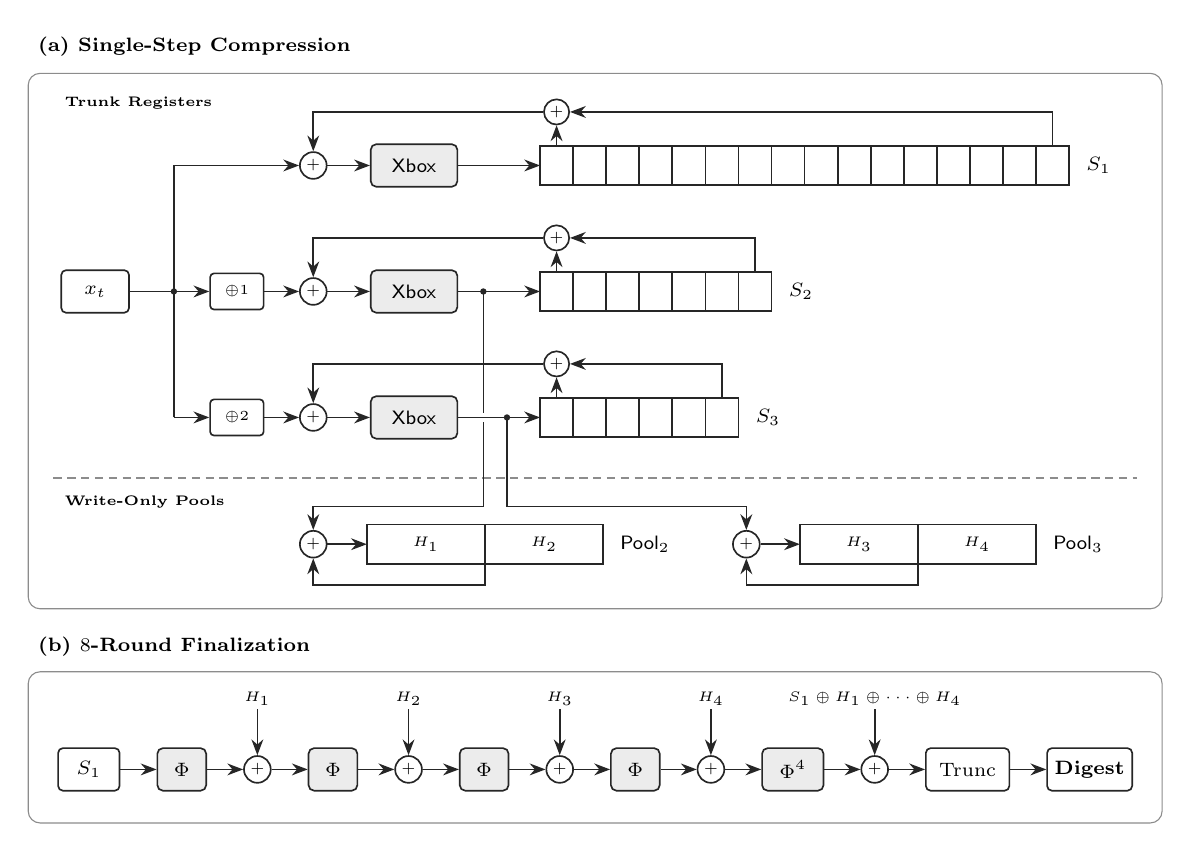
\begin{tikzpicture}[
    >=Stealth,
    xboxnode/.style={rectangle, draw=black!85, semithick, rounded corners=0.7mm, fill=gray!15, minimum width=11.0mm, minimum height=5.4mm, inner sep=2pt, font=\scriptsize\bfseries},
    phinode/.style={rectangle, draw=black!85, semithick, rounded corners=0.7mm, fill=gray!15, minimum width=6.2mm, minimum height=5.4mm, inner sep=1.5pt, font=\scriptsize\bfseries},
    psinode/.style={rectangle, draw=black!85, semithick, rounded corners=0.7mm, fill=gray!15, minimum width=7.8mm, minimum height=5.4mm, inner sep=1.5pt, font=\scriptsize\bfseries},
    wbox/.style={rectangle, draw=black!85, semithick, rounded corners=0.6mm, fill=white, minimum height=5.4mm, inner sep=2pt, font=\scriptsize},
    cbox/.style={rectangle, draw=black!85, semithick, rounded corners=0.5mm, fill=white, minimum width=6.8mm, minimum height=4.6mm, inner sep=1.5pt, font=\tiny},
    xor/.style={circle, draw=black!85, semithick, fill=white, minimum size=3.4mm, inner sep=0pt, font=\tiny},
    txor/.style={circle, draw=black!85, semithick, fill=white, minimum size=3.2mm, inner sep=0pt, font=\tiny},
    lbl/.style={font=\scriptsize, inner sep=1.5pt},
    tlbl/.style={font=\tiny, inner sep=1.2pt},
    wire/.style={->, semithick, draw=black!85},
    lineonly/.style={semithick, draw=black!85}
]

% ================= PANEL (a): SINGLE-STEP COMPRESSION =================
\node[font=\scriptsize\bfseries, anchor=west] at (0.00, 5.16) {(a) Single-Step Compression};

\begin{scope}[on background layer]
    \draw[rounded corners=1.5mm, draw=black!45, fill=white] (0.00, -1.98) rectangle (14.40, 4.82);
\end{scope}

% Region labels above and below the one-way dashed boundary
\node[font=\tiny\bfseries, anchor=west] at (0.34, 4.44) {Trunk Registers};
\node[font=\tiny\bfseries, anchor=west] at (0.34, -0.62) {Write-Only Pools};

% Input word x_t and fan-out bus
\node[wbox, minimum width=8.6mm, font=\scriptsize\bfseries] (xt) at (0.85, 2.05) {$x_t$};
\coordinate (bus_top) at (1.85, 3.65);
\coordinate (bus_mid) at (1.85, 2.05);
\coordinate (bus_bot) at (1.85, 0.45);
\draw[lineonly] (xt.east) -- (bus_mid);
\draw[lineonly] (bus_bot) -- (bus_top);
\fill[black!85] (bus_mid) circle (1.15pt);

% --- STREAM 1 (16 cells, y = 3.65) ---
\node[xor]      (xor1) at (3.62, 3.65) {$+$};
\node[xboxnode] (xb1)  at (4.90, 3.65) {$\Xbox$};
\draw[wire] (bus_top) -- (xor1);
\draw[wire] (xor1)    -- (xb1);
\draw[wire] (xb1.east) -- (6.50, 3.65);

\draw[semithick, draw=black!85, fill=white] (6.50, 3.40) rectangle (13.22, 3.90);
\foreach \k in {1,...,15} {
    \draw[semithick, draw=black!85] ({6.50 + 0.42*\k}, 3.40) -- ({6.50 + 0.42*\k}, 3.90);
}
\node[lbl, anchor=west] at (13.38, 3.65) {$S_1$};

\node[txor] (tx1) at (6.71, 4.33) {$+$};
\draw[wire] (6.71, 3.90)  -- (tx1.south);
\draw[wire] (13.01, 3.90) |- (tx1.east);
\draw[wire] (tx1.west)    -| (xor1.north);

% --- STREAM 2 (7 cells, y = 2.05) ---
\node[cbox]     (c2)   at (2.65, 2.05) {$\oplus 1$};
\node[xor]      (xor2) at (3.62, 2.05) {$+$};
\node[xboxnode] (xb2)  at (4.90, 2.05) {$\Xbox$};
\draw[wire] (bus_mid) -- (c2);
\draw[wire] (c2)      -- (xor2);
\draw[wire] (xor2)    -- (xb2);
\draw[wire] (xb2.east) -- (6.50, 2.05);

\draw[semithick, draw=black!85, fill=white] (6.50, 1.80) rectangle (9.44, 2.30);
\foreach \k in {1,...,6} {
    \draw[semithick, draw=black!85] ({6.50 + 0.42*\k}, 1.80) -- ({6.50 + 0.42*\k}, 2.30);
}
\node[lbl, anchor=west] at (9.60, 2.05) {$S_2$};

\node[txor] (tx2) at (6.71, 2.73) {$+$};
\draw[wire] (6.71, 2.30) -- (tx2.south);
\draw[wire] (9.23, 2.30) |- (tx2.east);
\draw[wire] (tx2.west)   -| (xor2.north);

% --- STREAM 3 (6 cells, y = 0.45) ---
\node[cbox]     (c3)   at (2.65, 0.45) {$\oplus 2$};
\node[xor]      (xor3) at (3.62, 0.45) {$+$};
\node[xboxnode] (xb3)  at (4.90, 0.45) {$\Xbox$};
\draw[wire] (bus_bot) -- (c3);
\draw[wire] (c3)      -- (xor3);
\draw[wire] (xor3)    -- (xb3);

% Pool_2 downward tap with crisp bridge over xb3->S_3 wire
\draw[semithick, densely dashed, draw=black!45] (0.32, -0.32) -- (14.08, -0.32);

\node[xor] (px2) at (3.62, -1.16) {$+$};
\node[xor] (px3) at (9.12, -1.16) {$+$};

\fill[black!85] (5.78, 2.05) circle (1.15pt);
\draw[wire] (5.78, 2.05) -- (5.78, -0.68) -| (px2.north);
\draw[white, line width=3.4pt] (5.64, 0.45) -- (5.92, 0.45);
\draw[wire] (xb3.east) -- (6.50, 0.45);

\fill[black!85] (6.08, 0.45) circle (1.15pt);
\draw[wire] (6.08, 0.45) -- (6.08, -0.68) -| (px3.north);

\draw[semithick, draw=black!85, fill=white] (6.50, 0.20) rectangle (9.02, 0.70);
\foreach \k in {1,...,5} {
    \draw[semithick, draw=black!85] ({6.50 + 0.42*\k}, 0.20) -- ({6.50 + 0.42*\k}, 0.70);
}
\node[lbl, anchor=west] at (9.18, 0.45) {$S_3$};

\node[txor] (tx3) at (6.71, 1.13) {$+$};
\draw[wire] (6.71, 0.70) -- (tx3.south);
\draw[wire] (8.81, 0.70) |- (tx3.east);
\draw[wire] (tx3.west)   -| (xor3.north);

% --- WRITE-ONLY ACCUMULATOR POOLS (y = -1.16) ---
\draw[semithick, draw=black!85, fill=white] (4.30, -1.41) rectangle (7.30, -0.91);
\draw[semithick, draw=black!85] (5.80, -1.41) -- (5.80, -0.91);
\node[tlbl] at (5.05, -1.16) {$H_1$};
\node[tlbl] at (6.55, -1.16) {$H_2$};
\draw[wire] (px2.east) -- (4.30, -1.16);
\draw[wire] (5.80, -1.41) -- (5.80, -1.68) -| (px2.south);
\node[lbl, anchor=west] at (7.46, -1.16) {$\Pool_2$};

\draw[semithick, draw=black!85, fill=white] (9.80, -1.41) rectangle (12.80, -0.91);
\draw[semithick, draw=black!85] (11.30, -1.41) -- (11.30, -0.91);
\node[tlbl] at (10.55, -1.16) {$H_3$};
\node[tlbl] at (12.05, -1.16) {$H_4$};
\draw[wire] (px3.east) -- (9.80, -1.16);
\draw[wire] (11.30, -1.41) -- (11.30, -1.68) -| (px3.south);
\node[lbl, anchor=west] at (12.96, -1.16) {$\Pool_3$};

% ================= PANEL (b): 8-ROUND FINALIZATION =================
\begin{scope}[yshift=-4.84cm]
    \node[font=\scriptsize\bfseries, anchor=west] at (0.00, 2.38) {(b) $8$-Round Finalization};

    \begin{scope}[on background layer]
        \draw[rounded corners=1.5mm, draw=black!45, fill=white] (0.00, 0.14) rectangle (14.40, 2.06);
    \end{scope}

    % Main horizontal pipeline at y = 0.82 (uniform 4.8 mm arrow shafts throughout)
    \node[wbox, minimum width=7.8mm] (w0)  at (0.77, 0.82) {$S_1$};
    \node[phinode]                   (f1)  at (1.95, 0.82) {$\Phi$};
    \node[xor]                       (p1)  at (2.91, 0.82) {$+$};
    \node[phinode]                   (f2)  at (3.87, 0.82) {$\Phi$};
    \node[xor]                       (p2)  at (4.83, 0.82) {$+$};
    \node[phinode]                   (f3)  at (5.79, 0.82) {$\Phi$};
    \node[xor]                       (p3)  at (6.75, 0.82) {$+$};
    \node[phinode]                   (f4)  at (7.71, 0.82) {$\Phi$};
    \node[xor]                       (p4)  at (8.67, 0.82) {$+$};
    \node[psinode]                   (psi) at (9.71, 0.82) {$\Phi^4$};
    \node[xor]                       (ff)  at (10.75, 0.82) {$+$};
    \node[wbox, minimum width=10.6mm] (tr) at (11.93, 0.82) {$\Trunc$};
    \node[wbox, minimum width=10.8mm, font=\scriptsize\bfseries] (dg) at (13.48, 0.82) {Digest};

    % Half-pool and feed-forward inputs from top (y = 1.72)
    \node[tlbl] (lp1) at (2.91, 1.72) {$H_1$};
    \node[tlbl] (lp2) at (4.83, 1.72) {$H_2$};
    \node[tlbl] (lp3) at (6.75, 1.72) {$H_3$};
    \node[tlbl] (lp4) at (8.67, 1.72) {$H_4$};
    \node[tlbl] (lff) at (10.75, 1.72) {$S_1 \oplus H_1 \oplus \cdots \oplus H_4$};

    \draw[wire] (w0)  -- (f1);
    \draw[wire] (f1)  -- (p1);  \draw[wire] (lp1) -- (p1);
    \draw[wire] (p1)  -- (f2);
    \draw[wire] (f2)  -- (p2);  \draw[wire] (lp2) -- (p2);
    \draw[wire] (p2)  -- (f3);
    \draw[wire] (f3)  -- (p3);  \draw[wire] (lp3) -- (p3);
    \draw[wire] (p3)  -- (f4);
    \draw[wire] (f4)  -- (p4);  \draw[wire] (lp4) -- (p4);
    \draw[wire] (p4)  -- (psi);
    \draw[wire] (psi) -- (ff);  \draw[wire] (lff) -- (ff);
    \draw[wire] (ff)  -- (tr);
    \draw[wire] (tr)  -- (dg);
\end{scope}

\end{tikzpicture}
\caption{Overall trunk-plus-accumulator architecture of Waterfall~\cite{Hat08}. \textbf{(a)}~Each compression step $\UpdateStep(\mathcal{S}, x_t)$ absorbs the $32$-bit input word $x_t$ ($16$ message words followed by block counter $\mathrm{ctr}_b = b \bmod 2^{32}$ every $17$-th step), updates the three cyclic trunk registers $S_1, S_2, S_3$ of coprime lengths $(16, 7, 6)$ via two-tap feedback and $\Xbox$, and XOR-accumulates the new outputs of $S_2$ and $S_3$ across a one-way write-only boundary into the $32$-word pools $\Pool_2 = (H_1, H_2)$ and $\Pool_3 = (H_3, H_4)$ at index $t \bmod 32$. \textbf{(b)}~The $8$-round finalization $\mathsf{Final}$ absorbs the four $16$-word half-pools $H_1, \dots, H_4$ into $S_1$ through $\Phi(W) = \Xbox^{\otimes 16}(L_{\mathrm{fin}}(W))$, applies $\Phi^4$, XORs the feed-forward sum $S_1 \oplus \bigoplus_{k=1}^4 H_k$, and truncates to $h/32$ words.}
\label{fig:waterfall-arch}
\end{figure}

\section{Full-State Collision Cryptanalysis}
\label{sec:collision}

We now present our unified algebraic differential collision framework, combining single-excursion pool cancellation, active counter-step message modification, and byte-cascade coset projection into a closed-form solver that reaches the minimal steerable single-excursion block lengths $B = 7$ ($448$ bytes) and $B = 8$ ($512$ bytes).

\subsection{Differential Fixed-Point Cosets of \texorpdfstring{$\Xbox$}{Xbox}}
\label{subsec:xbox-coset}

Our differential analysis follows the standard framework of Biham and Shamir~\cite{BihamShamir}, specialized to the inversion-based AES S-box~\cite{Nyberg}. For any word $Y \in \Ftwo^{32}$ and input difference $\alpha = (\alpha_0, \alpha_1, \alpha_2, \alpha_3) \in (\Ftwo^8)^4$, denote the $\Xbox$ output difference by
\[
\Phi_Y(\alpha) := \Xbox(Y) \oplus \Xbox(Y \oplus \alpha).
\]
Figure~\ref{fig:xbox-trail} depicts the $4$-round byte-cascade structure~\eqref{eq:XB-table}--\eqref{eq:xbox-def}. Write $Y = (b_0, b_1, b_2, b_3) \in (\Ftwo^8)^4$ and let $i_r \in \Ftwo^8$ denote the S-box input byte in micro-round $r \in \{1, 2, 3, 4\}$. Each micro-round then maps $(u_0, u_1, u_2, u_3) \mapsto (u_1 \oplus L_1(\Sbox(i_r)), \, u_2 \oplus L_2(\Sbox(i_r)), \, u_3 \oplus L_3(\Sbox(i_r)), \, \Sbox(i_r))$ with $i_r = u_0$. Now take a pair $(Y, Y \oplus \alpha)$ with S-box input differences $(\delta_1, \delta_2, \delta_3, \delta_4) \in (\Ftwo^8)^4$ and S-box output differences $(\Delta_1, \Delta_2, \Delta_3, \Delta_4) \in (\Ftwo^8)^4$ across the four micro-rounds. Any target output difference $\Delta w = \Phi_Y(\alpha) = (t_0, t_1, t_2, t_3) \in (\Ftwo^8)^4$ uniquely determines $(\Delta_1, \Delta_2, \Delta_3, \Delta_4)$ backward and $(\delta_1, \delta_2, \delta_3, \delta_4)$ forward via the linear triangular system:
\begin{align}
\Delta_4 &= t_3, \qquad \Delta_3 = t_2 \oplus \tilde{L}_3(\Delta_4), \qquad \Delta_2 = t_1 \oplus \tilde{L}_2(\Delta_4) \oplus \tilde{L}_3(\Delta_3), \nonumber \\
\Delta_1 &= t_0 \oplus \tilde{L}_1(\Delta_4) \oplus \tilde{L}_2(\Delta_3) \oplus \tilde{L}_3(\Delta_2), \label{eq:ds-back} \\
\delta_1 &= \alpha_0, \qquad \delta_2 = \alpha_1 \oplus \tilde{L}_1(\Delta_1), \qquad \delta_3 = \alpha_2 \oplus \tilde{L}_2(\Delta_1) \oplus \tilde{L}_1(\Delta_2), \nonumber \\
\delta_4 &= \alpha_3 \oplus \tilde{L}_3(\Delta_1) \oplus \tilde{L}_2(\Delta_2) \oplus \tilde{L}_1(\Delta_3). \label{eq:ek-fwd}
\end{align}
In particular, when $\alpha = \beta = (\beta_0, \beta_1, \beta_2, \mathtt{0x00})$ has top byte $\beta_3 = \mathtt{0x00}$, the top byte $b_3 \in \Ftwo^8$ of $Y = (b_0, b_1, b_2, b_3)$ does not enter the S-box during micro-rounds $r = 1, 2, 3$; instead, three applications of $\ROT$ shift $b_3$ into the fourth-round S-box input byte $i_4 = c_{3,0} \oplus b_3$, where $c_{3,0} \in \Ftwo^8$ denotes the low byte after three micro-rounds evaluated at $b_3 = 0$.

\begin{theorem}[Maximal $\Ftwo$-Affine Differential Fixed-Point Cosets of $\Xbox$]
\label{thm:xbox-coset}
For any non-zero difference $\beta = (\beta_0, \beta_1, \beta_2, \beta_3) \in (\Ftwo^8)^4 \setminus \{0\}$, define the differential fixed-point set
\[
T_\beta := \big\{ Y \in \Ftwo^{32} : \Phi_Y(\beta) = \beta \big\}.
\]
\begin{enumerate}[leftmargin=2em]
    \item \textbf{Closed-Form Size and Global Optimality:} For every non-zero $\beta$, the cardinality is $|T_\beta| = \prod_{r=1}^4 \mathsf{DDT}[\delta_r(\beta)][\Delta_r(\beta)]$. Since the AES S-box satisfies $\mathsf{DDT}[\delta][\Delta] \in \{0, 2, 4\}$ for $\delta \neq 0$ and $\mathsf{DDT}[0][0] = 256$, $|T_\beta|$ is maximized when one micro-round $r_0 \in \{1, 2, 3, 4\}$ is inactive ($\delta_{r_0}(\beta) = \Delta_{r_0}(\beta) = \mathtt{0x00}$) and the remaining three active micro-rounds realize $\{\mathsf{DDT}[\delta_r][\Delta_r]\}_{r \neq r_0} = \{2, 4, 4\}$. An exhaustive check over all $2^{32}-1$ non-zero differences confirms that the global maximum is
    \[
    \max_{\beta \neq 0} |T_\beta| = 2 \times 4 \times 4 \times 256 = 8{,}192 = 2^{13},
    \]
    attained by $8$ differences in $\Ftwo^{32}$ ($2$ for each $r_0 \in \{1, 2, 3, 4\}$), of which uniquely $\beta = \mathtt{0x00f9e70e}$ and $\beta' = \mathtt{0x003f7638}$ satisfy $r_0 = 4$ ($\beta_3 = \mathtt{0x00}$).
    \item \textbf{Direct-Sum $\Ftwo$-Affine Coset Structure:} Whereas the six maximizers with $r_0 \in \{1, 2, 3\}$ pass the unconstrained byte $i_{r_0}$ through $\Sbox$ before later rounds and form nonlinear $2^{13}$-element manifolds, for each of the two $r_0 = 4$ maximizers $\beta \in \{\mathtt{0x00f9e70e}, \mathtt{0x003f7638}\}$ the set $T_\beta$ is a \emph{single} $\Ftwo$-affine coset
    \[
    T_\beta = c \oplus V, \qquad V = H_{24} \oplus \mathcal{B}_3, \qquad \dim_{\Ftwo}(V) = 13, \qquad \beta \in H_{24},
    \]
    where $H_{24} \subset \Ftwo^{24} \times \{0\}$ is a $5$-dimensional low-$24$-bit subspace ($|H_{24}| = 32$) and $\mathcal{B}_3 = \{(0, 0, 0, b_3) : b_3 \in \Ftwo^8\} \subset (\Ftwo^8)^4$ is the unconstrained $8$-dimensional top-byte subspace.
    \item \textbf{$19$-Bit Linear Syndrome Characterization:} For $\beta \in \{\mathtt{0x00f9e70e}, \mathtt{0x003f7638}\}$, let $\sigma : \Ftwo^{32} \to \Ftwo^{19}$ denote the $\Ftwo$-linear quotient map modulo $V$ (supported entirely on the low $24$ bits of its input) and let $\tau = \sigma(c) \in \Ftwo^{19}$. Then for any $Y \in \Ftwo^{32}$,
    \begin{equation}
    \label{eq:syndrome-test}
    \Phi_Y(\beta) = \beta \quad \Longleftrightarrow \quad Y \in T_\beta \quad \Longleftrightarrow \quad \sigma(Y) = \tau.
    \end{equation}
\end{enumerate}
\end{theorem}
\begin{proof}
Setting $(t_0, t_1, t_2, t_3) = (\beta_0, \beta_1, \beta_2, \beta_3)$ in~\eqref{eq:ds-back}--\eqref{eq:ek-fwd} uniquely fixes $(\delta_r(\beta), \Delta_r(\beta))_{r=1}^4$. Because the map $Y \mapsto (i_1, i_2, i_3, i_4)$ is triangular and bijective over $(\Ftwo^8)^4$, $|T_\beta| = \prod_{r=1}^4 \mathsf{DDT}[\delta_r(\beta)][\Delta_r(\beta)]$. Since $\beta \neq 0$, not all four rounds can be inactive; if two or more rounds had $\Delta_r = 0$,~\eqref{eq:ds-back}--\eqref{eq:ek-fwd} can be checked directly across the $\binom{4}{2}\cdot(255)^2$ candidates to fall short of $2^{13}$, and an exhaustive $2^{32}$-word sweep confirms $\max_{\beta \neq 0}|T_\beta| = 2^{13}$ at $8$ differences ($2$ per $r_0$). When $r_0 = 4$, $\Delta_4 = \beta_3 = \mathtt{0x00}$ leaves $i_4$ unconstrained ($\mathsf{DDT}[0][0] = 256$). For the inversion-based AES S-box~\cite{Nyberg}, each active solution set $A_r = \{u \in \Ftwo^8 : \Sbox(u) \oplus \Sbox(u \oplus \delta_r) = \Delta_r\}$ ($r = 1, 2, 3$) is an $\Ftwo$-affine $1$- or $2$-flat, and on $A_1 \times A_2 \times A_3$ the S-box outputs $\Sbox(i_1), \Sbox(i_2)$ are $\Ftwo$-affine functions of $(i_1, i_2)$ (having dimension $\le 2$). Pulling $(A_1, A_2, A_3)$ back to $(b_0, b_1, b_2)$ therefore yields a $5$-dimensional $\Ftwo$-affine flat $c_0 \oplus H_{24}$ in $\Ftwo^{24}\times\{0\}$ with $\beta \in H_{24}$, while $b_3 \in \Ftwo^8$ never enters $i_1, i_2, i_3$. Part~(3) follows immediately from $\ker(\sigma) = V$.
\end{proof}

\begin{figure}[t!]
\centering
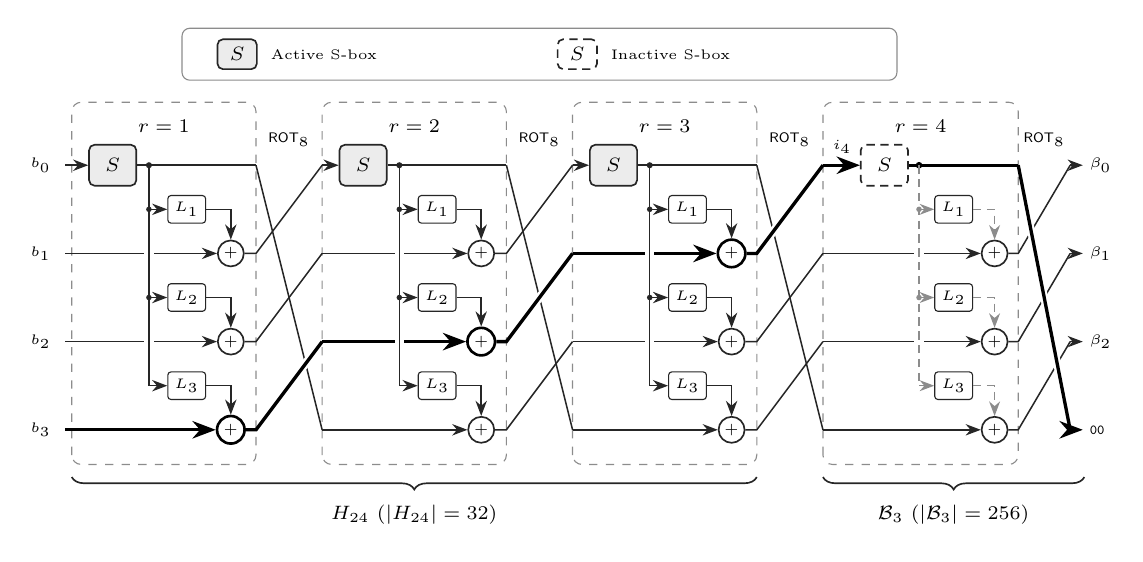
\begin{tikzpicture}[
    >=Stealth,
    sact/.style={rectangle, draw=black!85, semithick, rounded corners=0.7mm, fill=gray!15, minimum width=6.0mm, minimum height=5.2mm, inner sep=1.5pt, font=\scriptsize\bfseries},
    sinact/.style={rectangle, draw=black!85, semithick, densely dashed, rounded corners=0.7mm, fill=white, minimum width=6.0mm, minimum height=5.2mm, inner sep=1.5pt, font=\scriptsize\bfseries},
    lbox/.style={rectangle, draw=black!85, rounded corners=0.4mm, fill=white, minimum width=4.8mm, minimum height=3.5mm, inner sep=1pt, font=\tiny},
    xor/.style={circle, draw=black!85, semithick, fill=white, minimum size=3.3mm, inner sep=0pt, font=\tiny},
    gxor/.style={circle, draw=black, line width=0.95pt, fill=white, minimum size=3.5mm, inner sep=0pt, font=\tiny\bfseries},
    lbl/.style={font=\scriptsize, inner sep=1.5pt},
    tlbl/.style={font=\tiny, inner sep=1.2pt},
    actwire/.style={->, line width=0.55pt, draw=black!85},
    actline/.style={line width=0.55pt, draw=black!85},
    freewire/.style={->, line width=1.2pt, draw=black},
    freeline/.style={line width=1.2pt, draw=black},
    zerowire/.style={->, line width=0.5pt, densely dashed, draw=black!45}
]

% Top legend bar [2.60, 11.96]
\draw[rounded corners=1.0mm, draw=black!45, fill=white] (2.80, 4.44) rectangle (11.88, 5.10);
\node[sact, minimum width=5.0mm, minimum height=3.8mm, anchor=west] at (3.24, 4.77) {$S$};
\node[tlbl, anchor=west] at (3.88, 4.77) {Active S-box};
\node[sinact, minimum width=5.0mm, minimum height=3.8mm, anchor=west] at (7.56, 4.77) {$S$};
\node[tlbl, anchor=west] at (8.20, 4.77) {Inactive S-box};

% Input byte labels (right-aligned at x = 1.18)
\node[tlbl, anchor=east] at (1.18, 3.36) {$b_0$};
\node[tlbl, anchor=east] at (1.18, 2.24) {$b_1$};
\node[tlbl, anchor=east] at (1.18, 1.12) {$b_2$};
\node[tlbl, anchor=east, font=\tiny\bfseries] at (1.18, 0.00) {$b_3$};

% Background panels for micro-rounds r = 1, 2, 3, 4
\begin{scope}[on background layer]
    \foreach \xL/\wP in {1.40/2.34, 4.58/2.34, 7.76/2.34, 10.94/2.48} {
        \draw[rounded corners=1.2mm, dashed, draw=black!45, fill=white] (\xL, -0.44) rectangle ({\xL+\wP}, 4.16);
    }
\end{scope}

% Round headers (well above S-boxes at y = 3.36)
\node[lbl, font=\scriptsize\bfseries] at (2.57, 3.86) {$r = 1$};
\node[lbl, font=\scriptsize\bfseries] at (5.75, 3.86) {$r = 2$};
\node[lbl, font=\scriptsize\bfseries] at (8.93, 3.86) {$r = 3$};
\node[lbl, font=\scriptsize\bfseries] at (12.18, 3.86) {$r = 4$};

% Round 1 nodes
\node[sact] (sb1) at (1.92, 3.36) {$S$};
\node[lbox] (l1_1) at (2.86, 2.80) {$L_1$};
\node[lbox] (l2_1) at (2.86, 1.68) {$L_2$};
\node[lbox] (l3_1) at (2.86, 0.56) {$L_3$};
\node[xor]  (xr1_1) at (3.42, 2.24) {$+$};
\node[xor]  (xr2_1) at (3.42, 1.12) {$+$};
\node[gxor] (xr3_1) at (3.42, 0.00) {$+$};

% Round 2 nodes
\node[sact] (sb2) at (5.10, 3.36) {$S$};
\node[lbox] (l1_2) at (6.04, 2.80) {$L_1$};
\node[lbox] (l2_2) at (6.04, 1.68) {$L_2$};
\node[lbox] (l3_2) at (6.04, 0.56) {$L_3$};
\node[xor]  (xr1_2) at (6.60, 2.24) {$+$};
\node[gxor] (xr2_2) at (6.60, 1.12) {$+$};
\node[xor]  (xr3_2) at (6.60, 0.00) {$+$};

% Round 3 nodes
\node[sact] (sb3) at (8.28, 3.36) {$S$};
\node[lbox] (l1_3) at (9.22, 2.80) {$L_1$};
\node[lbox] (l2_3) at (9.22, 1.68) {$L_2$};
\node[lbox] (l3_3) at (9.22, 0.56) {$L_3$};
\node[gxor] (xr1_3) at (9.78, 2.24) {$+$};
\node[xor]  (xr2_3) at (9.78, 1.12) {$+$};
\node[xor]  (xr3_3) at (9.78, 0.00) {$+$};

% Round 4 nodes
\node[sinact] (sb4) at (11.72, 3.36) {$S$};
\node[lbox] (l1_4) at (12.60, 2.80) {$L_1$};
\node[lbox] (l2_4) at (12.60, 1.68) {$L_2$};
\node[lbox] (l3_4) at (12.60, 0.56) {$L_3$};
\node[xor]  (xr1_4) at (13.12, 2.24) {$+$};
\node[xor]  (xr2_4) at (13.12, 1.12) {$+$};
\node[xor]  (xr3_4) at (13.12, 0.00) {$+$};

% Entry into Round 1
\draw[actwire]  (1.32, 3.36) -- (sb1.west);
\draw[actwire]  (1.32, 2.24) -- (xr1_1.west);
\draw[actwire]  (1.32, 1.12) -- (xr2_1.west);
\draw[freewire] (1.32, 0.00) -- (xr3_1.west);

% Round 1 exit + ROT_8 (3.74 -> 4.58): b_3 shifts lane 3 -> lane 2
\draw[actline]  (xr1_1.east) -- (3.74, 2.24) -- (4.58, 3.36); \draw[actwire]  (4.58, 3.36) -- (sb2.west);
\draw[actline]  (xr2_1.east) -- (3.74, 1.12) -- (4.58, 2.24); \draw[actwire]  (4.58, 2.24) -- (xr1_2.west);
\draw[actline]  (3.74, 3.36) -- (4.58, 0.00);                 \draw[actwire]  (4.58, 0.00) -- (xr3_2.west);
\draw[white, line width=3.0pt] (4.24, 0.67) -- (4.42, 0.91);
\draw[freeline] (xr3_1.east) -- (3.74, 0.00) -- (4.58, 1.12); \draw[freewire] (4.58, 1.12) -- (xr2_2.west);
\node[tlbl] at (4.16, 3.68) {$\ROT$};

% Round 2 exit + ROT_8 (6.92 -> 7.76): b_3 shifts lane 2 -> lane 1
\draw[actline]  (xr1_2.east) -- (6.92, 2.24) -- (7.76, 3.36); \draw[actwire]  (7.76, 3.36) -- (sb3.west);
\draw[actline]  (xr3_2.east) -- (6.92, 0.00) -- (7.76, 1.12); \draw[actwire]  (7.76, 1.12) -- (xr2_3.west);
\draw[actline]  (6.92, 3.36) -- (7.76, 0.00);                 \draw[actwire]  (7.76, 0.00) -- (xr3_3.west);
\draw[white, line width=3.0pt] (7.22, 1.52) -- (7.40, 1.76);
\draw[freeline] (xr2_2.east) -- (6.92, 1.12) -- (7.76, 2.24); \draw[freewire] (7.76, 2.24) -- (xr1_3.west);
\node[tlbl] at (7.34, 3.68) {$\ROT$};

% Round 3 exit + ROT_8 (10.10 -> 10.94): b_3 shifts lane 1 -> lane 0 (S-box 4 input i_4)
\draw[actline]  (xr2_3.east) -- (10.10, 1.12) -- (10.94, 2.24); \draw[actwire]  (10.94, 2.24) -- (xr1_4.west);
\draw[actline]  (xr3_3.east) -- (10.10, 0.00) -- (10.94, 1.12); \draw[actwire]  (10.94, 1.12) -- (xr2_4.west);
\draw[actline]  (10.10, 3.36) -- (10.94, 0.00);                 \draw[actwire]  (10.94, 0.00) -- (xr3_4.west);
\draw[white, line width=3.0pt] (10.22, 2.40) -- (10.40, 2.64);
\draw[freeline] (xr1_3.east) -- (10.10, 2.24) -- (10.94, 3.36);
\draw[freewire] (10.94, 3.36) -- node[tlbl, above=2.5pt, pos=0.52, font=\tiny\bfseries] {$i_4$} (sb4.west);
\node[tlbl] at (10.52, 3.68) {$\ROT$};

% Vertical tap spines for Rounds 1, 2, 3 with crisp white-halo bridges over lanes 1 & 2
\foreach \r/\xtap/\xend in {1/2.38/3.74, 2/5.56/6.92, 3/8.74/10.10} {
    \draw[white, line width=3.4pt] (\xtap, 2.38) -- (\xtap, 2.10);
    \draw[white, line width=3.4pt] (\xtap, 1.26) -- (\xtap, 0.98);
    \draw[actline] (sb\r.east) -- (\xend, 3.36);
    \fill[black!85] (\xtap, 3.36) circle (1.1pt);
    \draw[actline] (\xtap, 3.36) -- (\xtap, 0.56);
    \fill[black!85] (\xtap, 2.80) circle (1.0pt);
    \fill[black!85] (\xtap, 1.68) circle (1.0pt);
    \draw[actwire] (\xtap, 2.80) -- (l1_\r.west);
    \draw[actwire] (\xtap, 1.68) -- (l2_\r.west);
    \draw[actwire] (\xtap, 0.56) -- (l3_\r.west);
    \draw[actwire] (l1_\r.east) -| (xr1_\r.north);
    \draw[actwire] (l2_\r.east) -| (xr2_\r.north);
    \draw[actwire] (l3_\r.east) -| (xr3_\r.north);
}

% Vertical tap spine for Round 4 (zero-difference dashed taps)
\draw[white, line width=3.4pt] (12.16, 2.38) -- (12.16, 2.10);
\draw[white, line width=3.4pt] (12.16, 1.26) -- (12.16, 0.98);
\draw[freeline] (sb4.east) -- (13.42, 3.36);
\fill[black] (12.16, 3.36) circle (1.2pt);
\draw[line width=0.5pt, densely dashed, draw=black!45] (12.16, 3.36) -- (12.16, 0.56);
\fill[black!45] (12.16, 2.80) circle (1.0pt);
\fill[black!45] (12.16, 1.68) circle (1.0pt);
\draw[zerowire] (12.16, 2.80) -- (l1_4.west);
\draw[zerowire] (12.16, 1.68) -- (l2_4.west);
\draw[zerowire] (12.16, 0.56) -- (l3_4.west);
\draw[zerowire] (l1_4.east) -| (xr1_4.north);
\draw[zerowire] (l2_4.east) -| (xr2_4.north);
\draw[zerowire] (l3_4.east) -| (xr3_4.north);

% Round 4 exit + final ROT_8 (13.42 -> 14.08)
\draw[actline]  (xr1_4.east) -- (13.42, 2.24) -- (14.08, 3.36); \draw[actwire]  (14.08, 3.36) -- (14.24, 3.36);
\draw[actline]  (xr2_4.east) -- (13.42, 1.12) -- (14.08, 2.24); \draw[actwire]  (14.08, 2.24) -- (14.24, 2.24);
\draw[actline]  (xr3_4.east) -- (13.42, 0.00) -- (14.08, 1.12); \draw[actwire]  (14.08, 1.12) -- (14.24, 1.12);
\draw[white, line width=2.8pt] (13.54, 2.75) -- (13.96, 0.61);
\draw[freeline] (13.42, 3.36) -- (14.08, 0.00);                 \draw[freewire] (14.08, 0.00) -- (14.24, 0.00);
\node[tlbl] at (13.75, 3.68) {$\ROT$};

% Output difference labels
\node[tlbl, anchor=west] at (14.28, 3.36) {$\beta_0$};
\node[tlbl, anchor=west] at (14.28, 2.24) {$\beta_1$};
\node[tlbl, anchor=west] at (14.28, 1.12) {$\beta_2$};
\node[tlbl, anchor=west, font=\tiny\bfseries] at (14.28, 0.00) {$\mathtt{00}$};

% Bottom braces explaining Theorem 1 and Theorem 3 simultaneously
\draw[decorate, decoration={brace, mirror, amplitude=4.5pt}, semithick, draw=black!85]
    (1.40, -0.60) -- (10.10, -0.60)
    node[midway, below=6.5pt, font=\scriptsize]
    {$H_{24}$ ($|H_{24}| = 32$)};

\draw[decorate, decoration={brace, mirror, amplitude=4.5pt}, semithick, draw=black!85]
    (10.94, -0.60) -- (14.26, -0.60)
    node[midway, below=6.5pt, font=\scriptsize]
    {$\mathcal{B}_3$ ($|\mathcal{B}_3| = 256$)};
\end{tikzpicture}
\caption{Byte-lane Generalized-Feistel structure of $\Xbox$ across its four micro-rounds ($r = 1, 2, 3, 4$) for a maximal fixed-point difference $\beta = (\beta_0, \beta_1, \beta_2, \mathtt{0x00})$ (Theorems~\ref{thm:xbox-coset} and~\ref{thm:byte-cascade}). Setting $\beta_3 = \delta_4 = \Delta_4 = \mathtt{0x00}$ leaves the fourth-round AES S-box inactive ($\mathsf{DDT}[0][0] = 256$), while the unconstrained top byte $b_3 \in \Ftwo^8$ (heavy bold staircase) shifts undisturbed along lanes $3 \to 2 \to 1 \to 0$ into $i_4 = c_{3,0} \oplus b_3$, yielding $|T_\beta| = 32 \times 256 = 2^{13}$ and enabling the $256\times$ coset-scan reduction.}
\label{fig:xbox-trail}
\end{figure}

\subsection{Pool Parity Cancellation and Counter Steering}
\label{subsec:pattern-counter}

Fix $\beta = \mathtt{0x00f9e70e}$ from Theorem~\ref{thm:xbox-coset} and restrict the difference of every message word and every trunk register word across a $T$-step prefix ($T = 17 B$) to the two-element alphabet $\{0, \beta\}$. Let $d_t \in \Ftwo$ indicate whether $\Delta x_t = \beta$, and let $(e_1[t], e_2[t], e_3[t]) := (u_t, v_t, w_t) \in \Ftwo^3$ indicate whether the words written into $S_1[t \bmod 16]$, $S_2[t \bmod 7]$, and $S_3[t \bmod 6]$ at step $t$ carry difference $\beta$.

Whenever every active stream at step $t$ satisfies the linear syndrome condition~\eqref{eq:syndrome-test}, $\Xbox$ acts as the identity on the difference $\beta$ ($\Phi_Y(\beta) = \beta$). As a result, the differential trajectory $(u_t, v_t, w_t)_{t=0}^{T-1}$ is governed by the exact $\Ftwo$-linear shift-register recurrences:
\begin{equation}
\label{eq:uvw-rec}
u_t = u_{t-1} \oplus u_{t-16} \oplus d_t, \qquad
v_t = v_{t-1} \oplus v_{t-7}  \oplus d_t, \qquad
w_t = w_{t-1} \oplus w_{t-6}  \oplus d_t,
\end{equation}
with $u_s = v_s = w_s = 0$ for $s < 0$. Using standard polynomial delay notation over $\Ftwo[x]$ for shift-register trails~\cite{RVP01,DaemenVanAssche},~\eqref{eq:uvw-rec} reads $(1 + x + x^{16})U(x) = (1 + x + x^7)V(x) = (1 + x + x^6)W(x) = D(x)$. Because the three feedback trinomials are pairwise coprime over $\Ftwo[x]$, finite-support trunk excursions correspond precisely to multiples $D(x) = L(x) Q(x)$ of the degree-$29$ generator polynomial
\begin{equation}
\label{eq:lcm-poly}
L(x) = \lcm\big(1 + x + x^{16}, \, 1 + x + x^7, \, 1 + x + x^6\big) = (1 + x + x^{16})(1 + x + x^7)(1 + x + x^6), \qquad \deg L = 29.
\end{equation}

A complete $93$-word internal state collision occurs at step $T$ if and only if both the $29$ trunk registers and the $64$ accumulator pool words return to zero difference:
\begin{enumerate}[leftmargin=2em]
    \item \textbf{Trunk Register Extinction:} The final $K_i$ steps of each stream write zero differences, overwriting every register slot:
    \begin{equation}
    \label{eq:tail-zero}
    u_t = 0 \;\;\forall t \in [T-16, T), \qquad
    v_t = 0 \;\;\forall t \in [T-7, T), \qquad
    w_t = 0 \;\;\forall t \in [T-6, T).
    \end{equation}
    \item \textbf{Single-Excursion In-Window Pool Parity Cancellation:} Every step $t$ with $v_t = 1$ (resp.\ $w_t = 1$) XORs the \emph{exact same difference $\beta$} into $\Pool_2[t \bmod 32]$ (resp.\ $\Pool_3[t \bmod 32]$). Repeating a register excursion twice at a step offset $\Delta s \equiv 0 \pmod{\lcm(17, 32) = 544}$ (requiring $44$ blocks $= 2{,}816$ bytes) is therefore \emph{unnecessary}. Instead, all $64$ pool words cancel to zero difference within a \emph{single excursion} if and only if each residue class $r \in \{0, \dots, 31\}$ is visited an even number of times:
    \begin{equation}
    \label{eq:pool-parity}
    \bigoplus_{\substack{0 \le t < T \\ t \equiv r \pmod{32}}} v_t = 0, \qquad
    \bigoplus_{\substack{0 \le t < T \\ t \equiv r \pmod{32}}} w_t = 0 \qquad \forall r \in \{0, 1, \dots, 31\}.
    \end{equation}
\end{enumerate}

\paragraph{Condition Accounting and Counter Steering.}
Recall the pre-input trunk tap sums $P_a(t), P_b(t), P_c(t)$ defined in~\eqref{eq:PaPbPc}, where $Y_a(t) = P_a(t) \oplus x_t$, $Y_b(t) = P_b(t) \oplus x_t \oplus 1$, and $Y_c(t) = P_c(t) \oplus x_t \oplus 2$. The pairwise inter-stream input differences
\begin{equation}
\label{eq:AtCtGt}
A_t := Y_a(t) \oplus Y_b(t) = P_a(t) \oplus P_b(t) \oplus 1, \quad
C_t := Y_a(t) \oplus Y_c(t) = P_a(t) \oplus P_c(t) \oplus 2, \quad
G_t := A_t \oplus C_t
\end{equation}
are \emph{completely independent of the current message word $x_t$}. Let $\mathrm{act}_t = u_t + v_t + w_t \in \{0, 1, 2, 3\}$ denote the number of active streams at step $t$, and let $T_0$ denote the unique initial \emph{injection step} where the first non-zero message difference $d_{T_0} = 1$ activates all three streams ($u_{T_0} = v_{T_0} = w_{T_0} = 1$):
\begin{itemize}[leftmargin=2em]
    \item \textbf{Message-Word Steps ($t \not\equiv 16 \pmod{17}$):}
    \begin{itemize}
        \item If $\mathrm{act}_t = 0$: $x_t \in \Ftwo^{32}$ is completely free ($32$ bits of freedom, $0$ conditions).
        \item If $\mathrm{act}_t = 1$: choosing $x_t$ in the $2^{13}$-coset $P_i(t) \oplus c_i \oplus c \oplus V$ satisfies $\sigma(Y_i(t)) = \tau$ automatically ($13$ neutral bits of freedom~\cite{BC04} in $V$, $0$ $x_t$-independent conditions).
        \item If $\mathrm{act}_t = 2$: $x_t$ absorbs one active stream, leaving one $x_t$-independent $19$-bit linear condition on the state entering step $t$: $A_t \in V$ (if $u_t = v_t = 1$), $C_t \in V$ (if $u_t = w_t = 1$), or $G_t \in V$ (if $v_t = w_t = 1$).
        \item If $\mathrm{act}_t = 3$ (at $t = T_0$): $x_{T_0}$ absorbs one stream, leaving two $x_{T_0}$-independent $19$-bit conditions ($A_{T_0} \in V$ and $C_{T_0} \in V$, $38$ bits in total), which we decouple across the four predecessor steps $T_0 - 4, \dots, T_0 - 1$ by pre-aligning $G_{T_0 - 2} = 0$ (Section~\ref{subsec:closed-form-walk}).
    \end{itemize}
    \item \textbf{Mandatory Block-Counter Steps ($t_{\mathrm{ctr}} \equiv 16 \pmod{17}$):} At any counter step $t = t_{\mathrm{ctr}}$, $d_t = 0$ and the input word is fixed to $\mathrm{ctr}_t = (\lfloor t / 17 \rfloor + 1) \bmod 2^{32}$. Forcing $u_t = v_t = w_t = 0$ at every counter step restricts $3$-step look-back steerable single-excursion patterns to $B \ge 9$ blocks ($576$ bytes). We break this $9$-block barrier by combining single-excursion pool parity cancellation~\eqref{eq:pool-parity} with active block-counter message modification~\cite{WangYu05} ($\mathrm{act}_t \le 1$ at $t \equiv 16 \pmod{17}$, illustrated in Figure~\ref{fig:collision-steering}). When a single stream $i \in \{1, 2, 3\}$ is active at counter step $t = t_{\mathrm{ctr}}$, it imposes a single $19$-bit condition $\sigma(P_i(t) \oplus \mathrm{ctr}_t \oplus c_i) = \tau$. Here $P_i(t) = \Xbox(Y_i(t-1)) \oplus S_i[t \bmod K_i]$, where $S_i[(t-1)\bmod K_i] = \Xbox(Y_i(t-1))$ is written at step $t - 1$ and $S_i[t \bmod K_i] = \Xbox(Y_i(t_{\mathrm{pre}}))$ was written $K_i$ steps earlier at $t_{\mathrm{pre}} = t - K_i$. The counter condition is satisfied in closed form via two mechanisms:
    \begin{enumerate}
        \item \textbf{Immediate Predecessor Modification ($e_i[t-1] = 0$):} When step $t - 1$ has $\mathrm{act}_{t-1} = 0$, $Y_i(t-1)$ is unconstrained, so setting
        \begin{equation}
        \label{eq:ctr-inv}
        Y_i(t-1) \leftarrow \Xbox^{-1}\!\big(S_i[t \bmod K_i] \oplus \mathrm{ctr}_t \oplus c_i \oplus c\big)
        \end{equation}
        satisfies $Y_i(t) = c \in T_\beta$ deterministically in $O(1)$ using a single $\Xbox^{-1}$ evaluation. When $\mathrm{act}_{t-1} = 1$ on a distinct stream $p \neq i$, $Y_i(t-1)$ is steered across the $32$-element low-$24$-bit coset of step $t - 1$.
        \item \textbf{Delayed Ring-Buffer Pre-Steering ($e_i[t-1] = 1$):} Suppose the same stream $i$ is active at both step $t - 1$ and counter step $t$. The recurrence $e_i[t] = e_i[t-1] \oplus e_i[t - K_i] \oplus d_t$ with $d_t = 0$ guarantees that $e_i[t_{\mathrm{pre}}] = 0$, so stream $i$ is inactive at step $t_{\mathrm{pre}} = t - K_i$. Fixing $Y_i(t-1) = c \in T_\beta$ at step $t - 1$ fixes $S_i[(t-1)\bmod K_i] = \Xbox(c)$, transferring the counter condition backward to step $t_{\mathrm{pre}} = t - K_i$:
        \begin{equation}
        \label{eq:ring-preset}
        \Xbox\big(Y_i(t_{\mathrm{pre}})\big) \in \big(\Xbox(c) \oplus \mathrm{ctr}_t \oplus c_i \oplus c\big) \oplus V,
        \end{equation}
        which is discharged at step $t_{\mathrm{pre}} = t - K_i$ via a precomputed counter-syndrome lookup table $\mathcal{T}_{\mathrm{ctr}}$ (Theorem~\ref{thm:byte-cascade}) before the walk reaches step $t$.
    \end{enumerate}
\end{itemize}

\begin{figure}[t!]
\centering
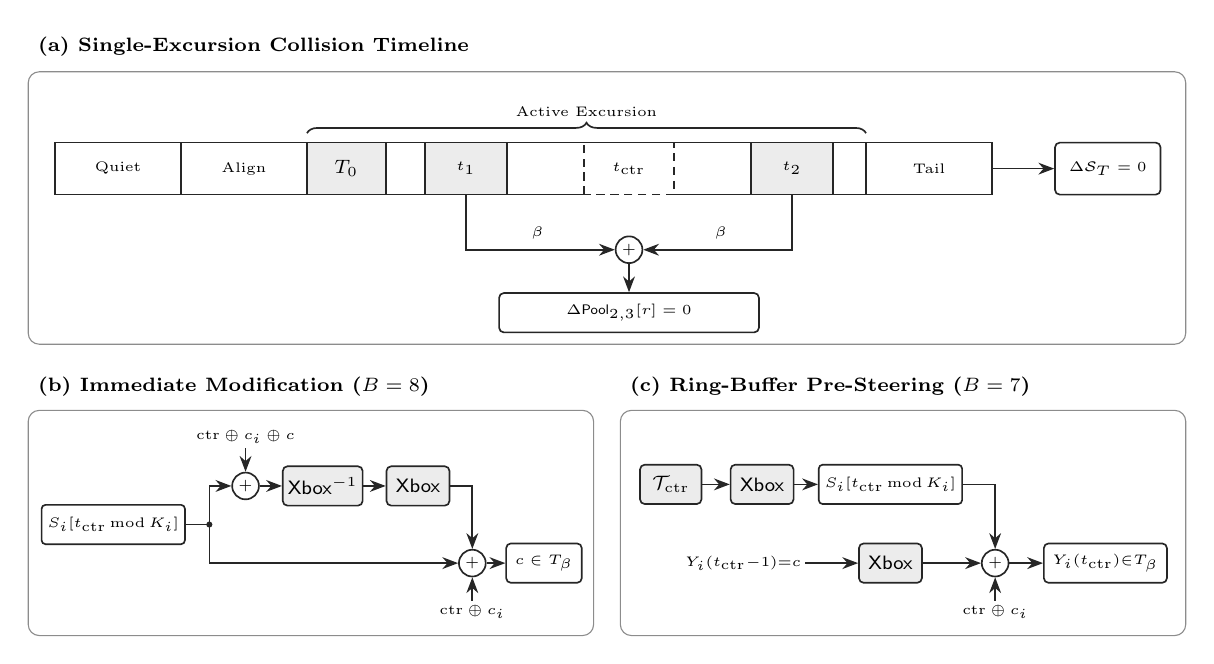
\begin{tikzpicture}[
    >=Stealth,
    xboxnode/.style={rectangle, draw=black!85, semithick, rounded corners=0.6mm, fill=gray!15, minimum width=8.0mm, minimum height=5.0mm, inner sep=1.8pt, font=\scriptsize\bfseries},
    xbinv/.style={rectangle, draw=black!85, semithick, rounded corners=0.6mm, fill=gray!15, minimum width=9.4mm, minimum height=5.0mm, inner sep=1.8pt, font=\scriptsize\bfseries},
    tblnode/.style={rectangle, draw=black!85, semithick, rounded corners=0.6mm, fill=gray!15, minimum width=7.8mm, minimum height=5.0mm, inner sep=1.8pt, font=\scriptsize\bfseries},
    slotbox/.style={rectangle, draw=black!85, semithick, rounded corners=0.5mm, fill=white, minimum width=15.4mm, minimum height=5.0mm, inner xsep=2.2pt, inner ysep=1.5pt, font=\tiny},
    resbox/.style={rectangle, draw=black!85, semithick, rounded corners=0.6mm, fill=white, minimum height=5.0mm, inner xsep=3.2pt, inner ysep=1.8pt, font=\tiny\bfseries},
    xor/.style={circle, draw=black!85, semithick, fill=white, minimum size=3.4mm, inner sep=0pt, font=\tiny},
    tlbl/.style={font=\tiny, inner sep=1.4pt},
    wire/.style={->, semithick, draw=black!85}
]

% ================= PANEL (a): SINGLE-EXCURSION COLLISION TIMELINE =================
\node[font=\scriptsize\bfseries, anchor=west] at (0.00, 3.92) {(a) Single-Excursion Collision Timeline};
\begin{scope}[on background layer]
    \draw[rounded corners=1.4mm, draw=black!45, fill=white] (0.00, 0.14) rectangle (14.70, 3.60);
\end{scope}

% Timeline bar across y in [2.04, 2.70] (height 0.66cm)
% Seg 1: Quiet prefix [0, T0-4)
\draw[semithick, draw=black!85, fill=white] (0.34, 2.04) rectangle (1.94, 2.70);
\node[tlbl] at (1.14, 2.37) {Quiet};

% Seg 2: 4-step alignment [T0-4, T0)
\draw[semithick, draw=black!85, fill=white] (1.94, 2.04) rectangle (3.54, 2.70);
\node[tlbl] at (2.74, 2.37) {Align};

% Seg 3: T0 injection step
\draw[semithick, draw=black!85, fill=gray!15] (3.54, 2.04) rectangle (4.54, 2.70);
\node[tlbl, font=\scriptsize\bfseries] at (4.04, 2.37) {$T_0$};

% Seg 4: Active Excursion Body [T0+1, T-16)
\draw[semithick, draw=black!85, fill=white] (4.54, 2.04) rectangle (10.64, 2.70);

% Paired residue steps t1 and t2 = t1 + 32k, plus counter step t_ctr
\draw[semithick, draw=black!85, fill=gray!15] (5.04, 2.04) rectangle (6.08, 2.70);
\node[tlbl, font=\tiny\bfseries] at (5.56, 2.37) {$t_1$};

\draw[semithick, densely dashed, draw=black!85, fill=white] (7.06, 2.04) rectangle (8.20, 2.70);
\node[tlbl, font=\tiny\bfseries] at (7.63, 2.37) {$t_{\mathrm{ctr}}$};

\draw[semithick, draw=black!85, fill=gray!15] (9.18, 2.04) rectangle (10.22, 2.70);
\node[tlbl, font=\tiny\bfseries] at (9.70, 2.37) {$t_2$};

% Brace over active excursion [T0, T-16)
\draw[semithick, draw=black!85, decorate, decoration={brace, amplitude=3.8pt}]
    (3.54, 2.82) -- node[tlbl, above=4.2pt] {Active Excursion} (10.64, 2.82);

% Seg 5: Tail Extinction [T-16, T)
\draw[semithick, draw=black!85, fill=white] (10.64, 2.04) rectangle (12.24, 2.70);
\node[tlbl] at (11.44, 2.37) {Tail};

% Final collision state at step T = 17B
\node[resbox, minimum width=1.34cm, minimum height=0.66cm] (finT) at (13.71, 2.37) {$\Delta \mathcal{S}_T = 0$};
\draw[wire] (12.24, 2.37) -- (finT.west);

% Modulo-32 Pool Parity Cancellation below body
\node[xor] (pcx) at (7.63, 1.34) {$+$};
\node[rectangle, draw=black!85, semithick, rounded corners=0.6mm, fill=white, minimum width=3.30cm, minimum height=0.50cm, inner xsep=5pt, inner ysep=2pt, font=\tiny] (pcell) at (7.63, 0.54) {$\Delta \Pool_{2,3}[r] = 0$};
\draw[wire] (5.56, 2.04) |- node[tlbl, above=2pt, pos=0.74] {$\beta$} (pcx.west);
\draw[wire] (9.70, 2.04) |- node[tlbl, above=2pt, pos=0.74] {$\beta$} (pcx.east);
\draw[wire] (pcx.south) -- (pcell.north);

% ================= PANEL (b): IMMEDIATE PREDECESSOR STEERING =================
\begin{scope}[yshift=-3.56cm, xshift=0.00cm]
    \node[font=\scriptsize\bfseries, anchor=west] at (0.00, 3.16) {(b) Immediate Modification ($B = 8$)};
    \draw[rounded corners=1.4mm, draw=black!45, fill=white] (0.00, 0.00) rectangle (7.18, 2.86);

    \node[slotbox] (b_slot) at (1.08, 1.41) {$S_i[t_{\mathrm{ctr}}\,\mathrm{mod}\,K_i]$};
    \fill[black!85] (2.30, 1.41) circle (1.1pt);
    \draw[semithick, draw=black!85] (b_slot.east) -- (2.30, 1.41);

    % Upper rail: step t_ctr - 1 inversion via Xbox^{-1}
    \node[xor]      (b_x0)  at (2.76, 1.90) {$+$};
    \node[tlbl]     (b_con) at (2.76, 2.52) {$\mathrm{ctr}\oplus c_i \oplus c$};
    \node[xbinv]    (b_inv) at (3.74, 1.90) {$\Xbox^{-1}$};
    \node[xboxnode] (b_xb)  at (4.95, 1.90) {$\Xbox$};

    \draw[wire] (2.30, 1.41) |- (b_x0.west);
    \draw[wire] (b_con.south) -- (b_x0.north);
    \draw[wire] (b_x0.east)  -- (b_inv.west);
    \draw[wire] (b_inv.east) -- (b_xb.west);

    % Lower rail: step t_ctr feed-forward cancellation
    \node[xor]  (b_xc)   at (5.64, 0.92) {$+$};
    \node[tlbl] (b_con2) at (5.64, 0.30) {$\mathrm{ctr}\oplus c_i$};
    \node[resbox, minimum width=8.2mm] (b_ok) at (6.55, 0.92) {$c \in T_\beta$};

    \draw[wire] (2.30, 1.41) |- (b_xc.west);
    \draw[wire] (b_xb.east)  -| (b_xc.north);
    \draw[wire] (b_con2.north) -- (b_xc.south);
    \draw[wire] (b_xc.east) -- (b_ok.west);
\end{scope}

% ================= PANEL (c): DELAYED RING-BUFFER PRE-STEERING =================
\begin{scope}[yshift=-3.56cm, xshift=7.52cm]
    \node[font=\scriptsize\bfseries, anchor=west] at (0.00, 3.16) {(c) Ring-Buffer Pre-Steering ($B = 7$)};
    \draw[rounded corners=1.4mm, draw=black!45, fill=white] (0.00, 0.00) rectangle (7.18, 2.86);

    % Upper rail: step t_pre = t_ctr - K_i pre-steering via T_ctr
    \node[tblnode]  (c_tbl)  at (0.64, 1.92) {$\mathcal{T}_{\mathrm{ctr}}$};
    \node[xboxnode] (c_xb1)  at (1.80, 1.92) {$\Xbox$};
    \node[slotbox]  (c_slot) at (3.43, 1.92) {$S_i[t_{\mathrm{ctr}}\,\mathrm{mod}\,K_i]$};

    \draw[wire] (c_tbl.east) -- (c_xb1.west);
    \draw[wire] (c_xb1.east) -- (c_slot.west);

    % Lower rail: step t_ctr - 1 pinned at c, combined at step t_ctr
    \node[tlbl, font=\tiny\bfseries] (pin_c)   at (1.56, 0.92) {$Y_i(t_{\mathrm{ctr}}{-}1){=}c$};
    \node[xboxnode]                  (xb_prev) at (3.43, 0.92) {$\Xbox$};
    \node[xor]                       (rxor)    at (4.76, 0.92) {$+$};
    \node[tlbl]                      (c_con)   at (4.76, 0.30) {$\mathrm{ctr}\oplus c_i$};
    \node[resbox]                    (rtarget) at (6.16, 0.92) {$Y_i(t_{\mathrm{ctr}}){\in}T_\beta$};

    \draw[wire] (pin_c.east)   -- (xb_prev.west);
    \draw[wire] (xb_prev.east) -- (rxor.west);
    \draw[wire] (c_slot.east)  -| (rxor.north);
    \draw[wire] (c_con.north)  -- (rxor.south);
    \draw[wire] (rxor.east)    -- (rtarget.west);
\end{scope}

\end{tikzpicture}
\caption{Single-excursion collision structure and active block-counter modification (Theorem~\ref{thm:min-blocks}). \textbf{(a)}~Across $T = 17B$ steps, the quiet prefix $[0, T_0 - 4)$ and $4$-step alignment $[T_0 - 4, T_0)$ prepare the $3$-stream injection at $T_0$ ($\Delta x_{T_0} = \beta$); inside the active excursion ($\Delta \in \{0, \beta\}$, mandatory counter steps $t_{\mathrm{ctr}} \equiv 16 \pmod{17}$ with $\Delta x_{t_{\mathrm{ctr}}} = 0$), residue-paired active steps $t_1 \equiv t_2 \equiv r \pmod{32}$ cancel every pool slot ($\beta \oplus \beta = 0$), and $[T - 16, T)$ extinguishes all $29$ trunk words to yield $\Delta \mathcal{S}_T = 0$. \textbf{(b)}~When $e_i[t_{\mathrm{ctr}}-1] = 0$, step $t_{\mathrm{ctr}} - 1$ applies $\Xbox^{-1}$ to cancel $S_i[t_{\mathrm{ctr}} \bmod K_i] \oplus \mathrm{ctr} \oplus c_i$ at step $t_{\mathrm{ctr}}$, placing $Y_i(t_{\mathrm{ctr}}) = c \in T_\beta$ ($B = 8$). \textbf{(c)}~When $e_i[t_{\mathrm{ctr}}-1] = 1$, $d_{t_{\mathrm{ctr}}} = 0$ forces $e_i[t_{\mathrm{pre}}] = 0$ at $t_{\mathrm{pre}} = t_{\mathrm{ctr}} - K_i$, pre-steering $S_i[t_{\mathrm{ctr}} \bmod K_i]$ via $\mathcal{T}_{\mathrm{ctr}}$ while pinning $Y_i(t_{\mathrm{ctr}}-1) = c$ ($B = 7$).}
\label{fig:collision-steering}
\end{figure}

To ensure that every step condition can be discharged sequentially without global multi-block backtracking, we call a trail $(d_t, u_t, v_t, w_t)_{t=0}^{T-1}$ \emph{$3$-step look-back steerable} if: (i)~it has a unique $3$-stream injection step $T_0 \ge 4$ preceded by four unconstrained ($\mathrm{act}_r = 0$) non-counter steps $T_0 - 4, \dots, T_0 - 1$, with $d_t = 0$ and $\mathrm{act}_t \le 1$ at every counter step $t \equiv 16 \pmod{17}$, $\mathrm{act}_{T_0 + 1} \le 1$, and $\mathrm{act}_t \le 2$ for all $t > T_0$; and (ii)~every subsequent step $t > T_0$ bearing an $x_t$-independent condition ($\mathrm{act}_t = 2$ at a non-counter step, or $\mathrm{act}_t = 1$ at a counter step $t \equiv 16 \pmod{17}$) has a non-counter predecessor $t - 1 \not\equiv 16 \pmod{17}$ and admits a non-counter step $s \in \{t - 1, t - 2, t - 3\} \cap (T_0, t)$ such that no step $r \in [s, t)$ bears an $x_r$-independent condition (i.e., $\mathrm{act}_r \le 1$ if $r \not\equiv 16 \pmod{17}$ and $\mathrm{act}_r = 0$ if $r \equiv 16 \pmod{17}$). (Without condition~(ii), the unconstrained linear system~\eqref{eq:uvw-rec}--\eqref{eq:pool-parity} already admits algebraic solutions at $B = 5$ blocks, but consecutive constrained steps create coupled multi-step nonlinear dependencies.)

\begin{theorem}[Minimal Steerable Single-Excursion Block Length for Waterfall]
\label{thm:min-blocks}
Among all $3$-step look-back steerable single-excursion trails satisfying~\eqref{eq:uvw-rec}, tail extinction~\eqref{eq:tail-zero}, and modulo-$32$ pool parity cancellation~\eqref{eq:pool-parity}:
\begin{enumerate}[leftmargin=2em]
    \item If active streams are forbidden on block-counter steps ($\mathrm{act}_t = 0$ for all $t \equiv 16 \pmod{17}$), all block lengths $B \le 8$ ($T \le 136$) are unsatisfiable, and the shortest steerable trail has $B = 9$ blocks ($576$ bytes, $T = 153$ steps).
    \item With active block-counter modification ($\mathrm{act}_t \le 1$ for $t \equiv 16 \pmod{17}$), block lengths $B \le 6$ ($T \le 102$, $\le 384$ bytes) are unsatisfiable, while $B = 8$ blocks ($512$ bytes, $T = 136$ steps) is satisfiable using immediate $O(1)$ counter inversion~\eqref{eq:ctr-inv}, and $B = 7$ blocks ($448$ bytes, $T = 119$ steps) is satisfiable and minimal among $3$-step look-back steerable trails using ring-buffer pre-steering~\eqref{eq:ring-preset}.
\end{enumerate}
\end{theorem}

\subsection{Closed-Form Step Recurrences and Coset Reduction}
\label{subsec:closed-form-walk}

We now show how the $x_t$-independent conditions $A_t \in V$, $C_t \in V$, and $G_t \in V$ of~\eqref{eq:AtCtGt} are solved in closed form without heuristic search. We also show how the direct-sum structure $V = H_{24} \oplus \mathcal{B}_3$ accelerates every constrained coset step by $256\times$.

\paragraph{Step-to-Step Difference Recurrences.}
At step $t$, define $z_t := P_a(t) \oplus x_t = Y_a(t) \in \Ftwo^{32}$, and define the three state-known constants entering step $t + 1$:
\[
\begin{aligned}
K_A(t) &:= S_1[(t+1)\bmod 16] \oplus S_2[(t+1)\bmod 7] \oplus 1, \\
K_C(t) &:= S_1[(t+1)\bmod 16] \oplus S_3[(t+1)\bmod 6] \oplus 2, \qquad
K_{AP}(t) := K_A(t) \oplus K_C(t).
\end{aligned}
\]
Because $Y_b(t) = z_t \oplus A_t$ and $Y_c(t) = z_t \oplus C_t$, the new words written at step $t$ satisfy $S_1[t\bmod 16] \oplus S_2[t\bmod 7] = \Xbox(z_t) \oplus \Xbox(z_t \oplus A_t) = \Phi_{z_t}(A_t)$, yielding the exact one-step recurrences:
\begin{equation}
\label{eq:ACG-rec}
\begin{aligned}
A_{t+1} &= \Phi_{z_t}(A_t) \oplus K_A(t), \\
C_{t+1} &= \Phi_{z_t}(C_t) \oplus K_C(t), \\
G_{t+1} &= \Phi_{z_t \oplus A_t}(G_t) \oplus K_{AP}(t).
\end{aligned}
\end{equation}

\paragraph{Decoupling the Three-Stream Injection Step.}
At the single $3$-stream injection step $T_0$, both $A_{T_0} \in V$ and $C_{T_0} \in V$ (equivalently, $G_{T_0} \in V$ and $C_{T_0} \in V$) must hold simultaneously ($38$ bits). Using four unconstrained predecessor steps $T_0 - 4, T_0 - 3, T_0 - 2, T_0 - 1$, the two $19$-bit conditions decouple completely in closed form:
\begin{enumerate}[leftmargin=2em]
    \item \textbf{Pre-Alignment ($G_{T_0 - 2} = 0$):} Using the closed-form differential constructor~\eqref{eq:ds-back}--\eqref{eq:ek-fwd}, choose $z_{T_0 - 4}$ so that $G_{T_0 - 3}$ lies in the solvable input-difference set of $K_{AP}(T_0 - 3)$, and then invert $\Phi_{\eta}(G_{T_0 - 3}) = K_{AP}(T_0 - 3)$ in $O(1)$ at step $T_0 - 3$ ($z_{T_0 - 3} = \eta \oplus A_{T_0 - 3}$), forcing $G_{T_0 - 2} = 0$, i.e., $A_{T_0 - 2} = C_{T_0 - 2} =: D$.
    \item \textbf{Decoupled Solve at $T_0 - 2$ and $T_0 - 1$:} Because $G_{T_0 - 2} = 0$ implies $\Phi_{z_{T_0 - 2} \oplus A_{T_0 - 2}}(0) = 0$, the state $G_{T_0 - 1} = K_{AP}(T_0 - 2)$ is \emph{independent of $z_{T_0 - 2}$}. We therefore first solve $\Phi_Z(G_{T_0 - 1}) \in K_{AP}(T_0 - 1) \oplus V$ for $Z = z_{T_0 - 1} \oplus A_{T_0 - 1}$, then solve $\Phi_{Z \oplus G_{T_0 - 1}}(C_{T_0 - 1}) \in K_C(T_0 - 1) \oplus V$ for the required difference $C_{T_0 - 1}$, and finally invert $\Phi_{z_{T_0 - 2}}(D) = C_{T_0 - 1} \oplus K_C(T_0 - 2)$ for $z_{T_0 - 2}$.
\end{enumerate}

\paragraph{Byte-Cascade Coset Reduction.}
At any $2$-stream step $t$,~\eqref{eq:ACG-rec} imposes a condition of the form $A_t = \Phi_{z_{t-1}}(D_0) \oplus K \in V$ with $D_0 = A_{t-1}$ and $K = K_A(t-1)$ (and similarly for $C_t$ or $G_t$). When $\mathrm{act}_{t-1} = 0$, $z_{t-1} \in \Ftwo^{32}$ is unconstrained, so we construct $z_{t-1}$ satisfying $\Phi_{z_{t-1}}(D_0) = K \oplus v$ (for the first admissible $v \in V$) in $O(1)$ via~\eqref{eq:ds-back}--\eqref{eq:ek-fwd}. When $\mathrm{act}_{t-1} = 1$, $z_{t-1}$ is restricted to a $2^{13}$-element coset $z_b \oplus V$. Rather than evaluating $\Phi_z(D_0)$ by brute force across all $2^{13} = 8{,}192$ elements $z \in z_b \oplus V$, we exploit the direct-sum decomposition $V = H_{24} \oplus \mathcal{B}_3$ of Theorem~\ref{thm:xbox-coset}.

\begin{theorem}[$32$-Element Byte-Cascade Coset Reduction]
\label{thm:byte-cascade}
Let $z = z_0 \oplus (0, 0, 0, b_3) \in z_b \oplus V$, where $z_0 \in z_{b,0} \oplus H_{24}$ (with $z_{b,0} = (b_0(z_b), b_1(z_b), b_2(z_b), 0)$) ranges over only $|H_{24}| = 32$ values and $(0, 0, 0, b_3) \in \mathcal{B}_3$ carries the unconstrained top byte $b_3 \in \Ftwo^8$. Let $w_0(z_0)$ and $w_1(z_0, D_0)$ denote the states of $z_0$ and $z_0 \oplus D_0$ after the first three micro-rounds of $\Xbox$ (evaluated at $b_3 = 0$), and let $c_{3,0} = b_0(w_0(z_0))$ and $c_{3,1} = b_0(w_1(z_0, D_0))$. Then:
\begin{enumerate}[leftmargin=2em]
    \item In micro-rounds $r = 1, 2, 3$, the S-box input bytes are independent of $b_3$, while after three right rotations $b_3$ shifts into the low byte (bits $0\text{--}7$) of both states, canceling in $w_0 \oplus w_1$ and shifting the fourth-round S-box index to $i_4 = c_{3,0} \oplus b_3$ with fixed input difference $\delta_4 = c_{3,0} \oplus c_{3,1}$.
    \item Therefore, the fourth-round S-box output difference $\Delta_4 = \Sbox(i_4) \oplus \Sbox(i_4 \oplus \delta_4)$ satisfies
    \[
    \begin{aligned}
    &\sigma\!\big(\Phi_{z_0 \oplus (0, 0, 0, b_3)}(D_0) \oplus K\big) = 0 \\
    \Longleftrightarrow \quad
    &\sigma\!\big(\ROT(\mathsf{XB}[i_4] \oplus \mathsf{XB}[i_4 \oplus \delta_4])\big) = \sigma\!\big(\ROT(w_0(z_0) \oplus w_1(z_0, D_0)) \oplus K\big).
    \end{aligned}
    \]
    Since $\sigma(\ROT(\mathsf{XB}[i_4] \oplus \mathsf{XB}[i_4 \oplus \delta_4]))$ depends exclusively on $\Delta_4 \in \Ftwo^8$ (as its top byte $\Delta_4 \oplus \delta_4$ lies in $\mathcal{B}_3 \subset V = \ker(\sigma)$), a precomputed syndrome-to-byte-difference lookup table $\mathcal{T}_{\Delta}$ recovers the unique candidate $\Delta_4$ in $O(1)$, and $b_3 = i_4 \oplus c_{3,0}$ exists if and only if $\mathsf{DDT}[\delta_4][\Delta_4] > 0$.
\end{enumerate}
Thus, solving $\Phi_z(D_0) \oplus K \in V$ over $z \in z_b \oplus V$ requires only $32$ three-round evaluations and $O(1)$ table lookups instead of $8{,}192$ four-round $\Xbox$ evaluations, achieving a $256\times$ reduction. The exact same $32$-element reduction applies to $1$-stream counter and ring-buffer pre-steering steps via a precomputed syndrome lookup table $\mathcal{T}_{\mathrm{ctr}}$ evaluated at $\tau \oplus \sigma(\ROT(w_0(y_0)) \oplus K_{\mathrm{ctr}})$.
\end{theorem}

\begin{figure}[t]
\centering
\small
\begin{tabular}{@{}p{0.97\textwidth}@{}}
\toprule
\textbf{Algorithm 1:} Unified Minimal-Length Full-State Collision Generator for Waterfall-$224/256/384/512$ \\
\midrule
\textbf{Input:} Target digest bit length $h \in \{224, 256, 384, 512\}$, block count $B \in \{7, 8, 9\}$ ($T = 17 B$), seed $s \ge 0$. \\
\textbf{Output:} Colliding $B$-block message pair $(M_1, M_2)$ ($M_1 \neq M_2$, $|M_1| = |M_2| = 64 B$ bytes) with identical $93$-word internal state at step $T$. \\[2pt]
\textbf{1.} Construct $T_\beta = c \oplus V$ for $\beta = \mathtt{0x00f9e70e}$ via~\eqref{eq:ds-back}--\eqref{eq:ek-fwd}, extract the $32$-element low-$24$-bit subspace $H_{24} \subset V$ and quotient map $\sigma : \Ftwo^{32} \to \Ftwo^{19}$, and precompute the $O(1)$ syndrome lookup tables $\mathcal{T}_{\Delta}$ and $\mathcal{T}_{\mathrm{ctr}}$. \\
\textbf{2.} Initialize state pair $(\mathcal{S}^{(1)}, \mathcal{S}^{(2)}) \leftarrow (\mathsf{Init}(h), \mathsf{Init}(h))$ and execute the $4$-step closed-form injection alignment at steps $T_0 - 4, \dots, T_0$ so that $A_{T_0}, C_{T_0} \in V$ and $\sigma(Y_a(T_0)) = \sigma(Y_b(T_0)) = \sigma(Y_c(T_0)) = \tau$. \\
\textbf{3.} \textbf{for} $t = T_0 + 1$ \textbf{to} $T - 1$ \textbf{do} \\
\hspace*{1.8em} \textbf{if} $t$ is a ring-buffer pre-steering step $t_{\mathrm{pre}} = t_{\mathrm{ctr}} - K_i$ for a counter step $t_{\mathrm{ctr}}$ with $e_i[t_{\mathrm{ctr}}] = e_i[t_{\mathrm{ctr}}-1] = 1$ \textbf{then} \\
\hspace*{3.6em} Steer $Y_i(t_{\mathrm{pre}})$ via $\mathcal{T}_{\mathrm{ctr}}$ so that $\Xbox(Y_i(t_{\mathrm{pre}})) \oplus \Xbox(c) \oplus \mathrm{ctr}_{t_{\mathrm{ctr}}} \oplus c_i \in c \oplus V$~\eqref{eq:ring-preset}. \\
\hspace*{1.8em} \textbf{else if} $t$ owns an $x_t$-independent $19$-bit condition ($\mathrm{act}_t = 2$ or counter step with $e_i[t-1] = 0$) \textbf{then} \\
\hspace*{3.6em} \textbf{if} $\mathrm{act}_{t-1} = 0$ \textbf{then} solve step $t - 1$ in $O(1)$ closed form via~\eqref{eq:ds-back}--\eqref{eq:ek-fwd} or $\Xbox^{-1}$~\eqref{eq:ctr-inv}. \\
\hspace*{3.6em} \textbf{else} redraw look-back word $x_{t-k}$ ($k \in \{2, 3\}$) and run the $32$-step byte-cascade solver via $\mathcal{T}_{\Delta}, \mathcal{T}_{\mathrm{ctr}}$ (Theorem~\ref{thm:byte-cascade}). \\
\hspace*{1.8em} Place $x_t^{(1)}$ in its admissible coset (or $x_t^{(1)} \leftarrow \mathrm{ctr}_t$ if $t \equiv 16 \pmod{17}$) and $x_t^{(2)} \leftarrow x_t^{(1)} \oplus d_t \beta$, advancing $(\mathcal{S}^{(1)}, \mathcal{S}^{(2)})$. \\
\textbf{4.} \textbf{return} the $64 B$-byte messages $M_1, M_2$ formed by the non-counter words $(x_t^{(1)})_{t \not\equiv 16}$ and $(x_t^{(2)})_{t \not\equiv 16}$. \\
\bottomrule
\end{tabular}
\end{figure}

\section{Security Analysis and Mitigations}
\label{sec:diagnosis}

\subsection{Flaws in the Design Security Argument}
The official Waterfall specification~\cite{Hat08} rested its collision security argument on three structural pillars. Our algebraic differential framework demonstrates that all three pillars collapse:
\begin{enumerate}[leftmargin=2em]
    \item \textbf{Failure of Coupled Stream Diffusion Over a Fixed-Point Coset:} Hattersley assumed that coupling three feedback streams of mutually coprime lengths $(16, 7, 6)$ through the nonlinear permutation $\Xbox$ would cause differences to avalanche uncontrollably across words and steps. However, $\Xbox$ is constructed as a $4$-round byte cascade where only one byte is substituted per micro-round. Choosing a difference $\beta$ with $\beta_3 = \mathtt{0x00}$ and $\delta_4(\beta) = \Delta_4(\beta) = \mathtt{0x00}$ therefore leaves the fourth-round S-box completely inactive ($\mathsf{DDT}[0][0] = 256$). This creates a $2^{13}$-element affine fixed-point coset $T_\beta = c \oplus V$ on which $\Xbox$ behaves as the \emph{identity map} on differences ($\Phi_Y(\beta) = \beta$). The three coupled nonlinear streams then become a linear code over $\Ftwo$, governed by the degree-$29$ generator polynomial $L(x) = \lcm(1+x+x^{16}, 1+x+x^7, 1+x+x^6)$ of~\eqref{eq:lcm-poly}.
    \item \textbf{Failure of the $17$-Step Block-Counter Defense:} Injecting the block counter $\mathrm{ctr}_b$ every $16$ message words was intended to prevent differential control at step $t \equiv 16 \pmod{17}$. The permutation $\Xbox$ is a bijection, and the register slot $S_i[(t-1)\bmod K_i]$ (resp.\ $S_i[t \bmod K_i]$) read at counter step $t$ is written at step $t - 1$ (resp.\ $t_{\mathrm{pre}} = t - K_i$). Any single-stream condition at a counter step is therefore satisfied in advance via message modification~\cite{WangYu05} using $\Xbox^{-1}$ and $\mathcal{T}_{\mathrm{ctr}}$~\eqref{eq:ctr-inv}--\eqref{eq:ring-preset}.
    \item \textbf{Failure of the Write-Only Accumulator Pools:} Because $\Pool_2$ and $\Pool_3$ are \emph{write-only} during message compression and never feed back into $S_1, S_2,$ or $S_3$, the trunk trajectory is completely blind to the pool state. When all active stream steps output the fixed difference $\beta$, all $64$ pool words cancel to zero difference within a single excursion via modulo-$32$ even parity~\eqref{eq:pool-parity}.
\end{enumerate}

\subsection{Structural Mitigations and Overhead}
To repair Waterfall's structural collision vulnerabilities, two modifications suffice:
\begin{enumerate}[leftmargin=2em]
    \item \textbf{Pool-to-Trunk Feedback During Absorption:} Add $\Pool_2[(t - \eta_1)\bmod 32]$ and $\Pool_3[(t - \eta_2)\bmod 32]$ (for fixed tap offsets $\eta_1, \eta_2$) into $Y_a(t), Y_b(t),$ and $Y_c(t)$ inside $\UpdateStep$, introducing pool-to-state feedback analogous to PANAMA~\cite{DC98}. This breaks the write-only isolation of the pools, preventing decoupled modulo-$32$ pool parity cancellation at a cost of two $32$-bit XORs per step ($\approx 3\%$ throughput overhead).
    \item \textbf{Full $4$-Byte Parallel Substitution and MDS Diffusion in $\Xbox$:} Replace the single-byte substitution $w \oplus \mathsf{XB}[b_0(w)]$ in each round of $\Xbox$ with a full $4$-byte parallel AES S-box layer followed by a $4 \times 4$ MDS matrix over $\mathbb{F}_{2^8}$ (branch number $5$, as in an AES column round~\cite{FIPSAES}). Because every two consecutive rounds then activate at least $5$ byte S-boxes ($\ge 10$ active S-boxes across four rounds), this eliminates inactive-S-box rounds and large affine fixed-point cosets.
\end{enumerate}

\section{Experimental Verification}
\label{sec:experiments}

All collision solvers were implemented in C with standard compiler optimizations on an Intel Xeon 6982P-C processor. We verified them offline against the unmodified official NIST SHA-3 Round~1 reference implementation~\cite{Hat08}.

\subsection{Collision Benchmarks and Component Ablations}
Table~\ref{tab:collision-bench} reports the single-core performance of our collision solvers across block lengths $B \in \{7, 8, 9\}$ ($448, 512,$ and $576$ bytes) and all four official NIST digest sizes ($h \in \{224, 256, 384, 512\}$). To isolate the impact of each technical contribution in Section~\ref{sec:collision}, we also evaluate two ablated configurations of our solver on Waterfall-$256$: disabling single-excursion pool parity cancellation~\eqref{eq:pool-parity} (repeating a quiet-counter excursion twice at step shift $\Delta s = 544$, $44$ blocks $= 2{,}816$ bytes), and disabling byte-cascade coset projection (scanning all $2^{13}$ coset elements on the $9$-block quiet-counter trail).

\begin{table}[t]
\centering
\caption{Single-core full-state collision benchmarks and component ablations of our framework, verified against the official NIST reference implementation~\cite{Hat08} (Xeon 6982P-C).}
\label{tab:collision-bench}
\footnotesize
\setlength{\tabcolsep}{2.4pt}
\begin{tabular}{@{}lccrrrll@{}}
\toprule
\textbf{Our Configuration} & \textbf{Blocks} & \textbf{Bytes} & \textbf{Steps} & \textbf{Active} & \textbf{Solve Time} & \textbf{Variants} & \textbf{Success} \\
\midrule
Dual-excursion (w/o Eq.~\eqref{eq:pool-parity}) & $44$ & $2{,}816$~B & $748$ & $36$ & $45.0$~ms & $256$ & $18 / 20$ ($90\%$) \\
$2^{13}$-coset scan (w/o Thm.~\ref{thm:byte-cascade}) & $9$ & $576$~B & $153$ & $50$ & $171.0$~ms & $256$ & $20 / 20$ ($100\%$) \\
\midrule
Quiet counter ($9$-block) & $9$ & $576$~B & $153$ & $50$ & $3.8$~ms & All $4$ & $20 / 20$ ($100\%$) \\
\textbf{Step $t{-}1$ mod.\ ($8$-block)} & $\mathbf{8}$ & $\mathbf{512}$~\textbf{B} & $136$ & $56$ & $\mathbf{3.5}$~\textbf{ms} & \textbf{All 4} & $\mathbf{20 / 20}$ ($\mathbf{100\%}$) \\
\textbf{Step $t{-}K_i$ pre-steering ($7$-block)} & $\mathbf{7}$ & $\mathbf{448}$~\textbf{B} & $119$ & $44$ & $\mathbf{52.1}$~\textbf{ms} & \textbf{All 4} & $\mathbf{20 / 20}$ ($\mathbf{100\%}$) \\
\bottomrule
\end{tabular}
\end{table}

\paragraph{$8$-Block ($512$-Byte) Solver.}
Our $8$-block solver succeeds on Attempt~$1$ across all $20$ tested seeds ($20/20$ distinct colliding pairs and digests), with a minimum runtime of $3.45$~ms and median of $4.26$~ms (mean $3.5$~ms, walk time $1.3$~ms), verified across Waterfall-$224, -256, -384,$ and $-512$. Enabling single-excursion pool cancellation~\eqref{eq:pool-parity} and immediate counter modification~\eqref{eq:ctr-inv} reduces message length by $5.5\times$ relative to our $44$-block dual-excursion configuration ($2{,}816$~B to $512$~B), while byte-cascade coset reduction (Theorem~\ref{thm:byte-cascade}) accelerates $9$-block solving by $45\times$ ($171.0$~ms to $3.8$~ms; $49\times$ to $3.5$~ms at $8$ blocks).

\paragraph{$7$-Block ($448$-Byte) Minimal Steerable Solver.}
Using delayed ring-buffer pre-steering~\eqref{eq:ring-preset} at step $t_{\mathrm{pre}} = 50 - 16 = 34$ for counter step $t_{\mathrm{ctr}} = 50$, together with immediate counter modification at $t_{\mathrm{ctr}} = 84$, our $7$-block solver generates verified $448$-byte full-state collisions in $52.1$~ms for Waterfall-$256$, matching the SAT lower bound for $3$-step look-back steerable trails ($B \le 6$ unsatisfiable). Across the remaining NIST digest sizes, the single-core solve times are $83.2$~ms (Waterfall-$224$), $290.8$~ms (Waterfall-$384$), and $126.0$~ms (Waterfall-$512$).

Table~\ref{tab:witness-fingerprints} summarizes the cryptographic fingerprints and official NIST Waterfall digests of our verified $448$-byte ($7$-block) and $512$-byte ($8$-block) collision pairs.

\begin{table}[t]
\centering
\caption{Cryptographic fingerprints of verified $448$-byte ($7$-block) and $512$-byte ($8$-block) full-state colliding message pairs $(M_1, M_2)$ for Waterfall-$256$.}
\label{tab:witness-fingerprints}
\footnotesize
\setlength{\tabcolsep}{4pt}
\begin{tabular}{@{}ll@{}}
\toprule
\textbf{Field} & \textbf{Verified Value (Hexadecimal)} \\
\midrule
\multicolumn{2}{@{}l}{\textbf{$7$-Block ($448$-Byte, $119$-Step) Full-State Collision Pair}} \\
$M_1$ SHA-256 & \texttt{11dd59480b379f12158d86466f4535fcc43d1172ed455a5cec62bcc5bc5f61c5} \\
$M_2$ SHA-256 & \texttt{9ad0f2ed6eb3188820e5dc19d9898351ec9009c76efbb69755a5bbe3100b32fd} \\
Waterfall-256 & \texttt{f1b0894f55696afb7e52b15ceb5e9f1c74d22d02a626e4b95a9f880cc45e5a29} \\
Active words & $44$ message words differing by $\beta = \mathtt{0x00f9e70e}$ \\
\midrule
\multicolumn{2}{@{}l}{\textbf{$8$-Block ($512$-Byte, $136$-Step) Full-State Collision Pair}} \\
$M_1$ SHA-256 & \texttt{a0c2fcb4a4cca44951ac764a5e7c39b11897e8eb1ed771f81dbd3b518d92174f} \\
$M_2$ SHA-256 & \texttt{579636a5831d61db67d526c89280a58eb2bdf23377f0311cf99d6bcf2445f341} \\
Waterfall-256 & \texttt{18a75611cd796ed22ff29a54db3f0e2a7cf6b9a25e5b065db9e8071fa4f482d2} \\
Active words & $56$ message words differing by $\beta = \mathtt{0x00f9e70e}$ \\
\bottomrule
\end{tabular}
\end{table}

\paragraph{Use of AI.}
The cryptanalytic results and artifacts were initially developed through an autonomous agent system powered by a MiniMax internal model. We validated the key technical claims and refined the presentation of the manuscript.

\begin{thebibliography}{99}

\bibitem{BDPA06}
G.~Bertoni, J.~Daemen, M.~Peeters, and G.~Van Assche,
``RadioGat\'{u}n, a Belt-and-Mill Hash Function,'' Presented at the NIST Second Cryptographic Hash Workshop, Santa Barbara, CA, Aug.~2006; Cryptology ePrint Archive, Paper 2006/369, 2006.

\bibitem{BC04}
E.~Biham and R.~Chen,
``Near-Collisions of SHA-0,'' in \emph{Advances in Cryptology -- CRYPTO 2004}, LNCS, vol.~3152, pp.~290--305, Springer, 2004.

\bibitem{BihamShamir}
E.~Biham and A.~Shamir,
``Differential Cryptanalysis of DES-like Cryptosystems,'' \emph{Journal of Cryptology}, vol.~4, no.~1, pp.~3--72, 1991.

\bibitem{Bra08}
C.~Bradbury,
``BLENDER: A Proposed New Family of Cryptographic Hash Algorithms,'' Algorithm Specification and Supporting Documentation, Submission to the NIST SHA-3 Competition (Round~1), Oct.~2008.

\bibitem{DC98}
J.~Daemen and C.~Clapp,
``Fast Hashing and Stream Encryption with PANAMA,'' in \emph{Fast Software Encryption -- FSE'98}, LNCS, vol.~1372, pp.~60--74, Springer, 1998.

\bibitem{DaemenVanAssche}
J.~Daemen and G.~Van Assche,
``Producing Collisions for Panama, Instantaneously,'' in \emph{Fast Software Encryption -- FSE 2007}, LNCS, vol.~4593, pp.~1--18, Springer, 2007.

\bibitem{Flu08}
S.~Fluhrer,
``Collision Attack on the Waterfall Hash Function,'' Cryptology ePrint Archive, Paper 2008/531, Dec.~2008.

\bibitem{Hat08}
B.~Hattersley,
``Waterfall Hash --- Algorithm Specification and Analysis,'' Version~1.0, Submission to the NIST SHA-3 Competition (Round~1), Oct.~15, 2008.

\bibitem{Hat08b}
B.~Hattersley,
``OFFICIAL COMMENT: Waterfall is broken,'' Official Public Comment, NIST SHA-3 Competition (Round~1), Dec.~20, 2008.

\bibitem{FIPSAES}
National Institute of Standards and Technology,
``Advanced Encryption Standard (AES),'' Federal Information Processing Standards Publication FIPS~PUB~197, Nov.~26, 2001.

\bibitem{SHAThreeCall}
National Institute of Standards and Technology,
``Announcing Request for Candidate Algorithm Nominations for a New Cryptographic Hash Algorithm (SHA-3) Family,'' \emph{Federal Register}, vol.~72, no.~212, pp.~62212--62220, Nov.~2, 2007.

\bibitem{Nyberg}
K.~Nyberg,
``Differentially Uniform Mappings for Cryptography,'' in \emph{Advances in Cryptology -- EUROCRYPT'93}, LNCS, vol.~765, pp.~55--64, Springer, 1994.

\bibitem{SHAThreeStatus}
A.~Regenscheid, R.~Perlner, S.-j.~Chang, J.~Kelsey, M.~Nandi, and S.~Paul,
``Status Report on the First Round of the SHA-3 Cryptographic Hash Algorithm Competition,'' NIST Interagency Report 7620, Sep.~2009.

\bibitem{RVP01}
V.~Rijmen, B.~Van Rompay, B.~Preneel, and J.~Vandewalle,
``Producing Collisions for PANAMA,'' in \emph{Fast Software Encryption -- FSE 2001}, LNCS, vol.~2355, pp.~37--51, Springer, 2002.

\bibitem{Str08}
M.~Trojnara,
``StreamHash Algorithm Specifications and Supporting Documentation,'' Submission to the NIST SHA-3 Competition (Round~1), Oct.~2008.

\bibitem{WangYu05}
X.~Wang and H.~Yu,
``How to Break MD5 and Other Hash Functions,'' in \emph{Advances in Cryptology -- EUROCRYPT 2005}, LNCS, vol.~3494, pp.~19--35, Springer, 2005.

\end{thebibliography}

\end{document}
